\section{Trigger and Instrumentation}
\label{chap:TriggerAndInstrumentation}

\subsection{Jet \pT Ranges}
\label{sec:ptRanges}

The selected jet \pT ranges for \pp collisions are as follows:

\begin{itemize}
    \item R = 0.2 $\rightarrow$ 20 - 240 GeV/c
    \item R = 0.3 $\rightarrow$ 20 - 240 GeV/c
    \item R = 0.4 $\rightarrow$ 20 - 240 GeV/c
    \item R = 0.5 $\rightarrow$ 20 - 160 GeV/c
\end{itemize}

The selected jet \pT range for \pPb collisions is as follows:

\begin{itemize}
    \item R = 0.2 $\rightarrow$ 20 - 240 GeV/c
    \item R = 0.3 $\rightarrow$ 20 - 240 GeV/c
    \item R = 0.4 $\rightarrow$ 20 - 120 GeV/c
\end{itemize}

The lower limit was selected based on the kinematic efficiency (see section \ref{subsec:kinEff}), while the upper limit was based on several criteria. First, the variation of the maximum track and cluster \pT cuts is studied. For more details and plots on this topic, see the systematics chapter \ref{chap:Systematics}. Once the max track/cluster cuts cause the spectrum to diverge significantly, the spectrum can no longer be trusted. This happens for all radii at 240 GeV/c. Next, the statistics must be considered. The response matrix is filtered at \pT-hard bin level to set any bins with less than 10 entries to zero. The unfolded spectrum produced by the filtered response is compared to the spectrum produced with the unfiltered response. The variation of the spectra is well within the statistical uncertainties within the chosen ranges listed above, and thus, the measurements can be trusted within these ranges. Ratio plots for this study can be found in appendix \ref{sec:appendixFilterComparison}. The upper limit for the largest radii was ultimately truncated at the point when the unfolding process was no longer stable.

\subsection{Event and Trigger Selection}
\label{sec:EvtTrgSel}

For the analysis, both minimum bias and EMCal triggers were used. For \pp, the min bias trigger covers the low jet-p$_T$ range from 20 - 30 GeV/c, while for higher jet-p$_T$, EMCal-L0 (EMC7) and L1 jet (EJE) triggers were used. These triggers cover 30 - 60 GeV/c and over 60 GeV/c, respectively. For \pPb, the min bias trigger covers the range from 20-30 GeV/c, while the two EMCal-L1 jet triggers, EJ2 and EJ1, cover the ranges 30 - 50 GeV/c and over 50 GeV, respectively.  These ranges were chosen based on the turn-on for each EMCal trigger. Once an adequate trigger efficiency is reached, and the trigger has reached the threshold in which it is bias-free, the trigger may be used (see section \ref{sec:EMCTriggerBias} for more details).

The \pp data for all triggers in this analysis were collected in 2012, and include periods LHC12a - LHC12i. The \pPb data for all trigger in this analysis were collected in 2016, and include periods LHC16r and LHC16s. From these periods, runs were selected for use only if the EMCal was read out and the data in the EMCAL was considered "good" (see appendix \ref{sec:goodRuns} for runlists corresponding to each period). These criteria excluded periods LHC12e and LHC12g. LHC12a and LHC12b were used only for the minimum bias trigger and were thus excluded from the analysis. Table~\ref{table:dataset_lumi} shows the integrated luminosity for each trigger used for the analysis.

Corrections from simulation were obtained using the production LHC16c2, a PYTHIA 8 simulation generated at \sNN = 8 TeV, using 20 bins of p$_T^{hard}$. The simulation was anchored to a number of runs in different periods in 2012, relative to the number of INT7 triggers in data.

A detailed QA was done on each period in data, both for the entire period and run-wise, and comparisons to simulation were performed \cite{JIRATicket}.

\begin{table}[hbt!]
    \centering
    \caption{Integrated luminosities for the \pp and \pPb datasets with downscale corrections.}
    \begin{tabular}{  m{2.4cm}  m{3cm} m{3cm}  }
        \hline
        System & Trigger Name & $\mathscr{L}_{\text{int}}  (\text{nb}^{-1})$ \\
        \hline
        \pp & INT7 & 0.968 \\
            & EMC7 & 41.4 \\
            & EJE & 588 \\ 
        \hline
        \pPb & INT7 & 7.35$\times 10^{-3}$ \\
             & EJ2 & 6.57$\times 10^{-2}$ \\
             & EJ1 & 1.34 \\ 
        \hline
    \end{tabular}
    \label{table:dataset_lumi}
  \end{table}

\subsection{Bias of the EMCal Trigger}
\label{sec:EMCTriggerBias}

The two EMCal triggers are based on the neutral component of the jet, and are implemented as a sliding window over the EMCal surface with two different patch sizes and energy thresholds:

\begin{itemize}
    \item EMC7: Threshold of 2 GeV, patch size of 2x2 cells
    \item EJE: Threshold of 16 GeV, patch size of 16x16 cells
    \item EJ2: Threshold of 18 GeV, patch size of 16x16 cells
    \item EJ1: Threshold of 23 GeV, patch size of 16x16 cells
\end{itemize}

\begin{figure}[h!]
    \centering
    \begin{multicols}{2}
            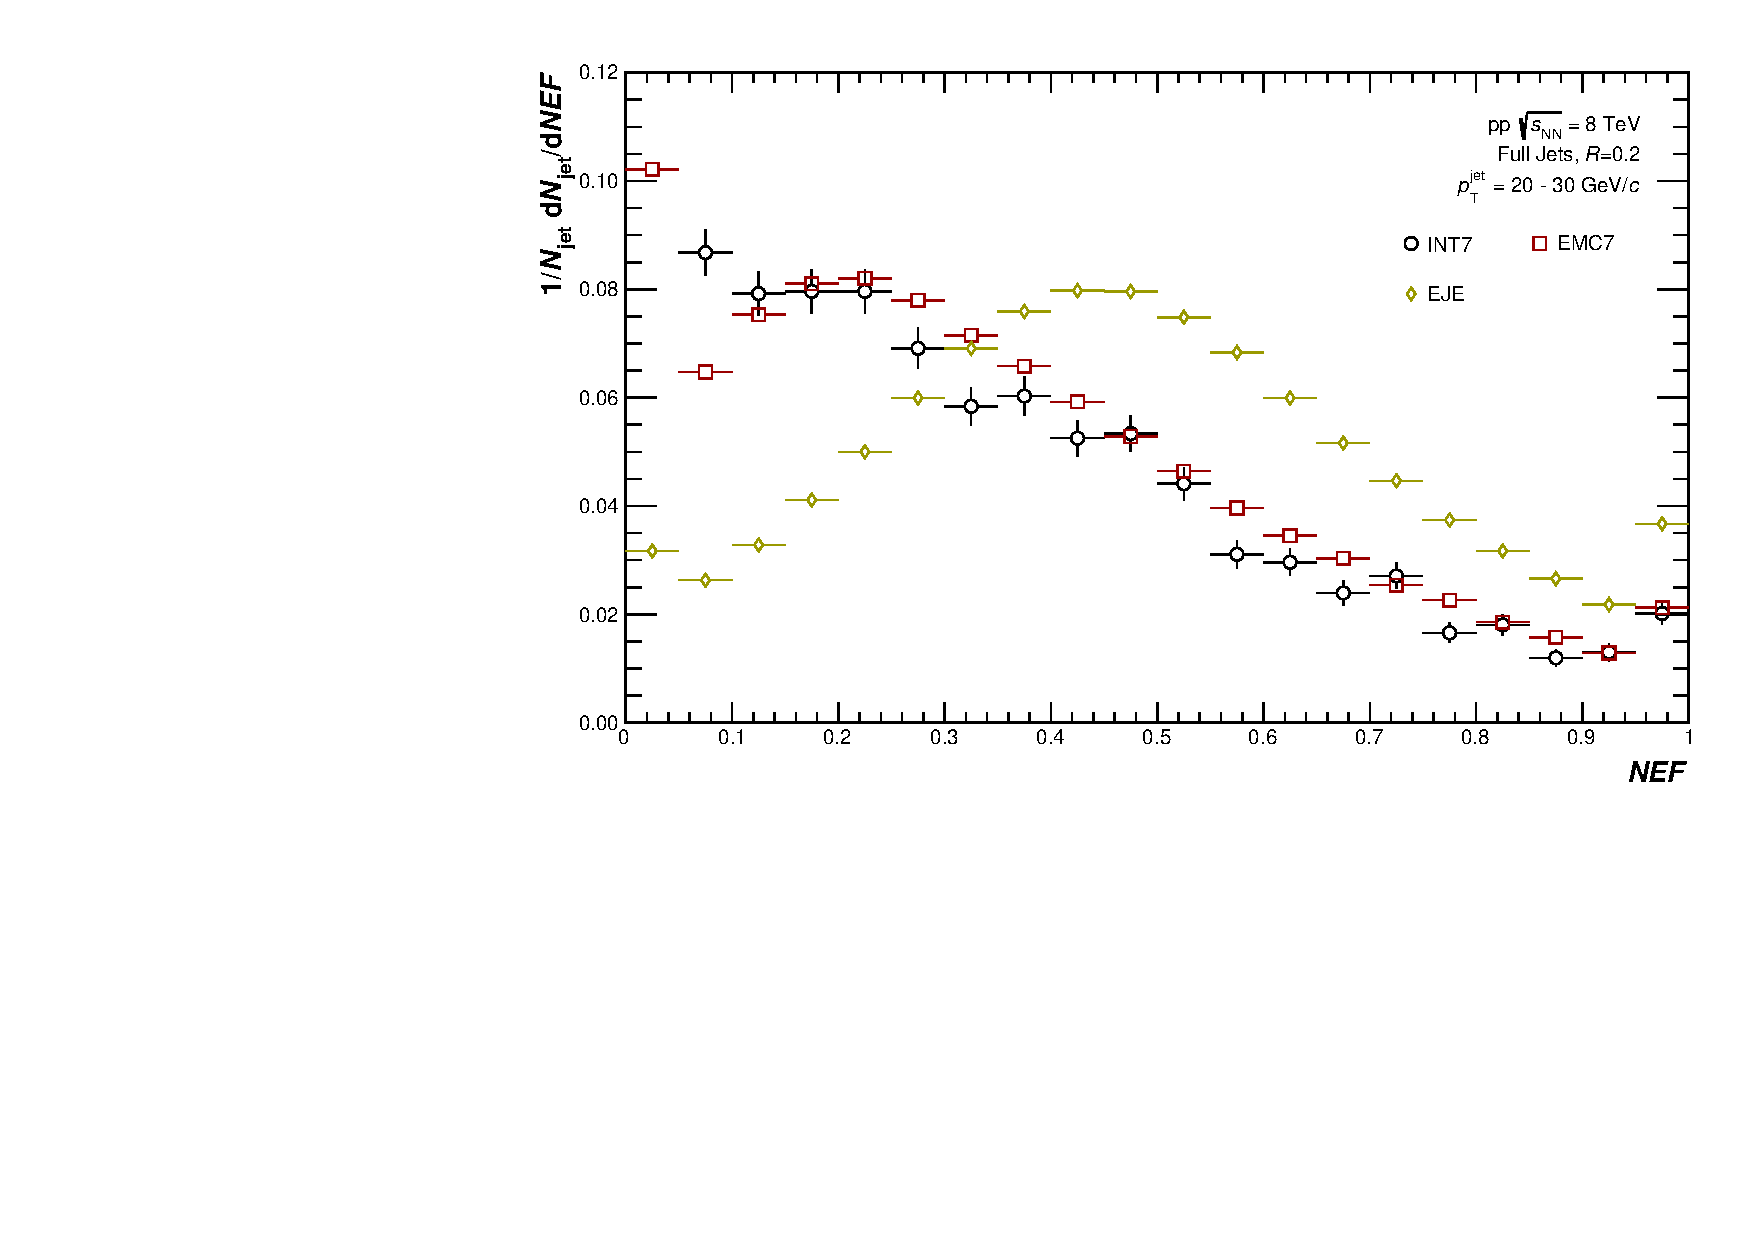
\includegraphics[width=7.5cm]{figures/NEF/All/hNEF_20-30GeV_R02.pdf}
            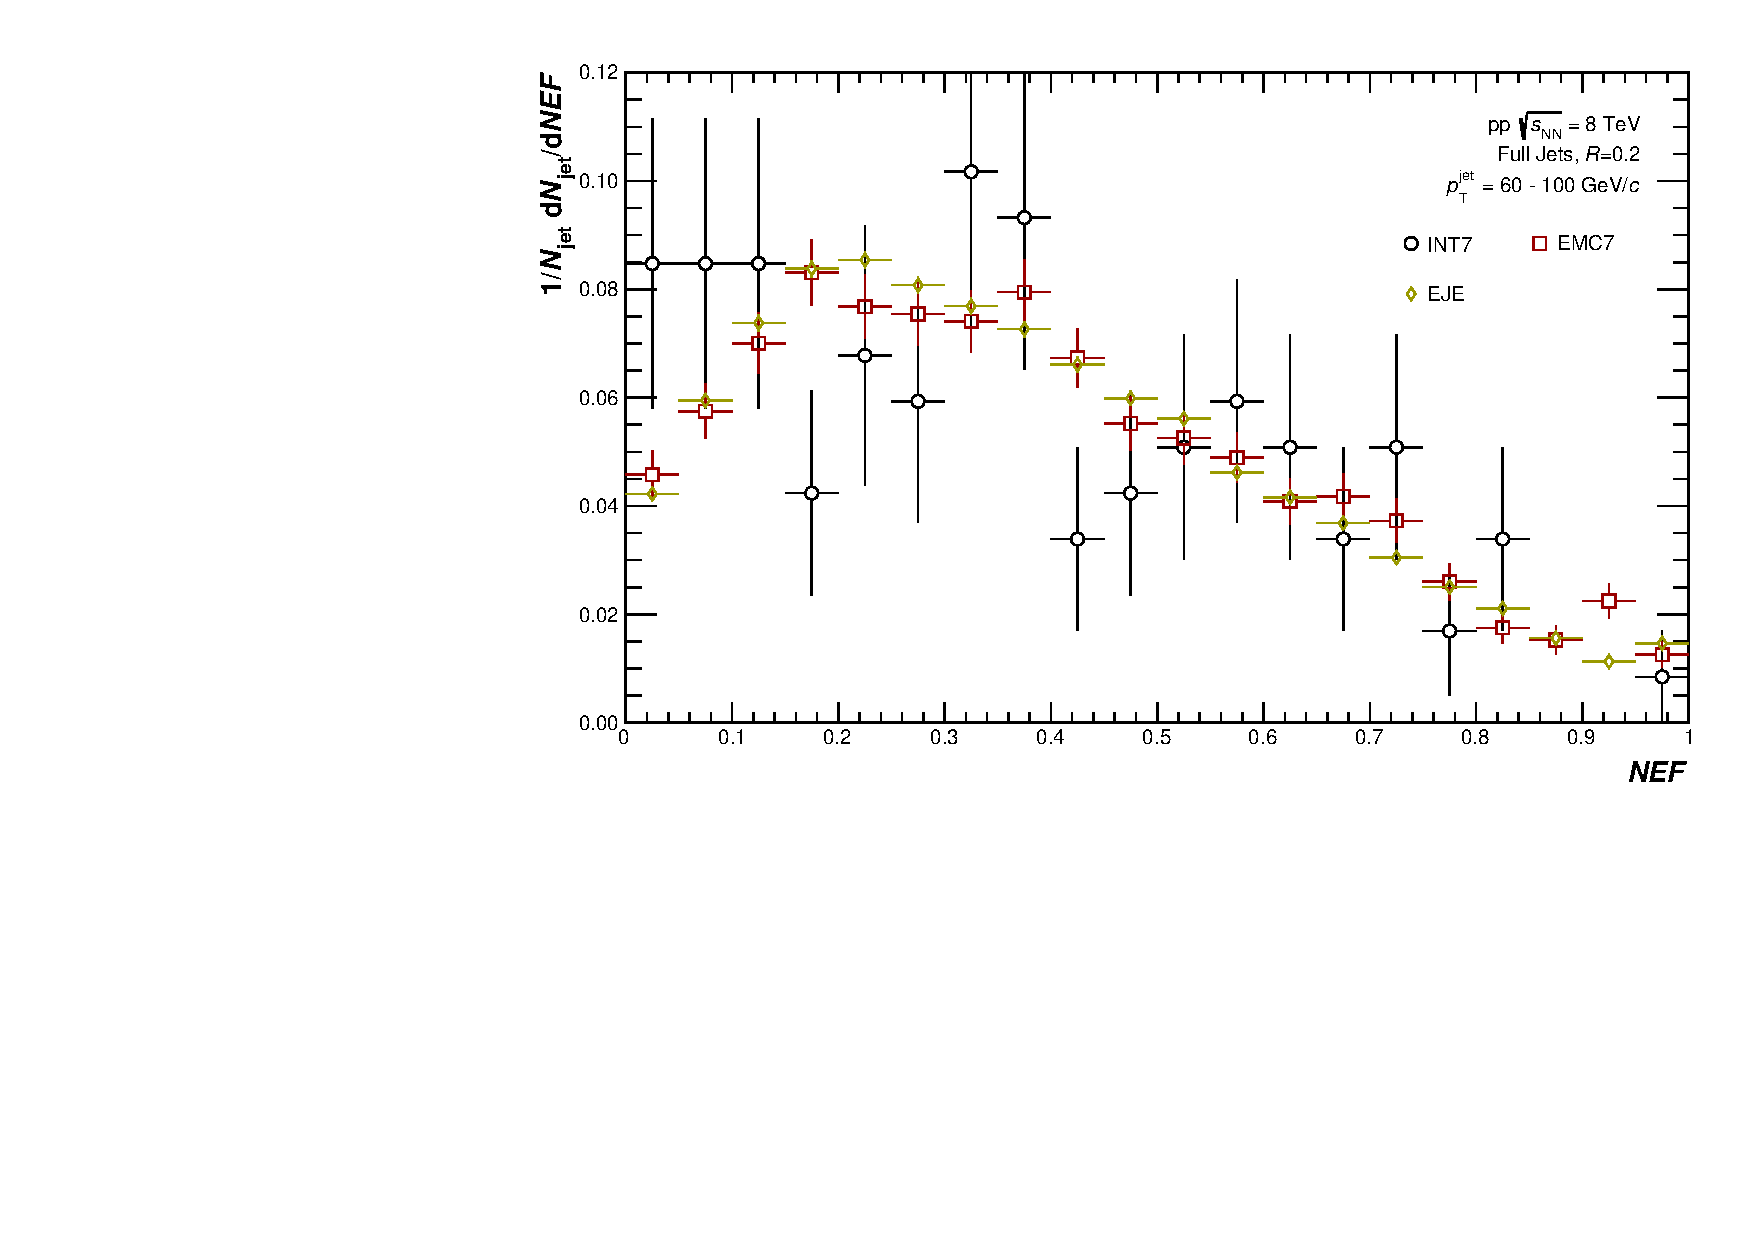
\includegraphics[width=7.5cm]{figures/NEF/All/hNEF_60-100GeV_R02.pdf}
            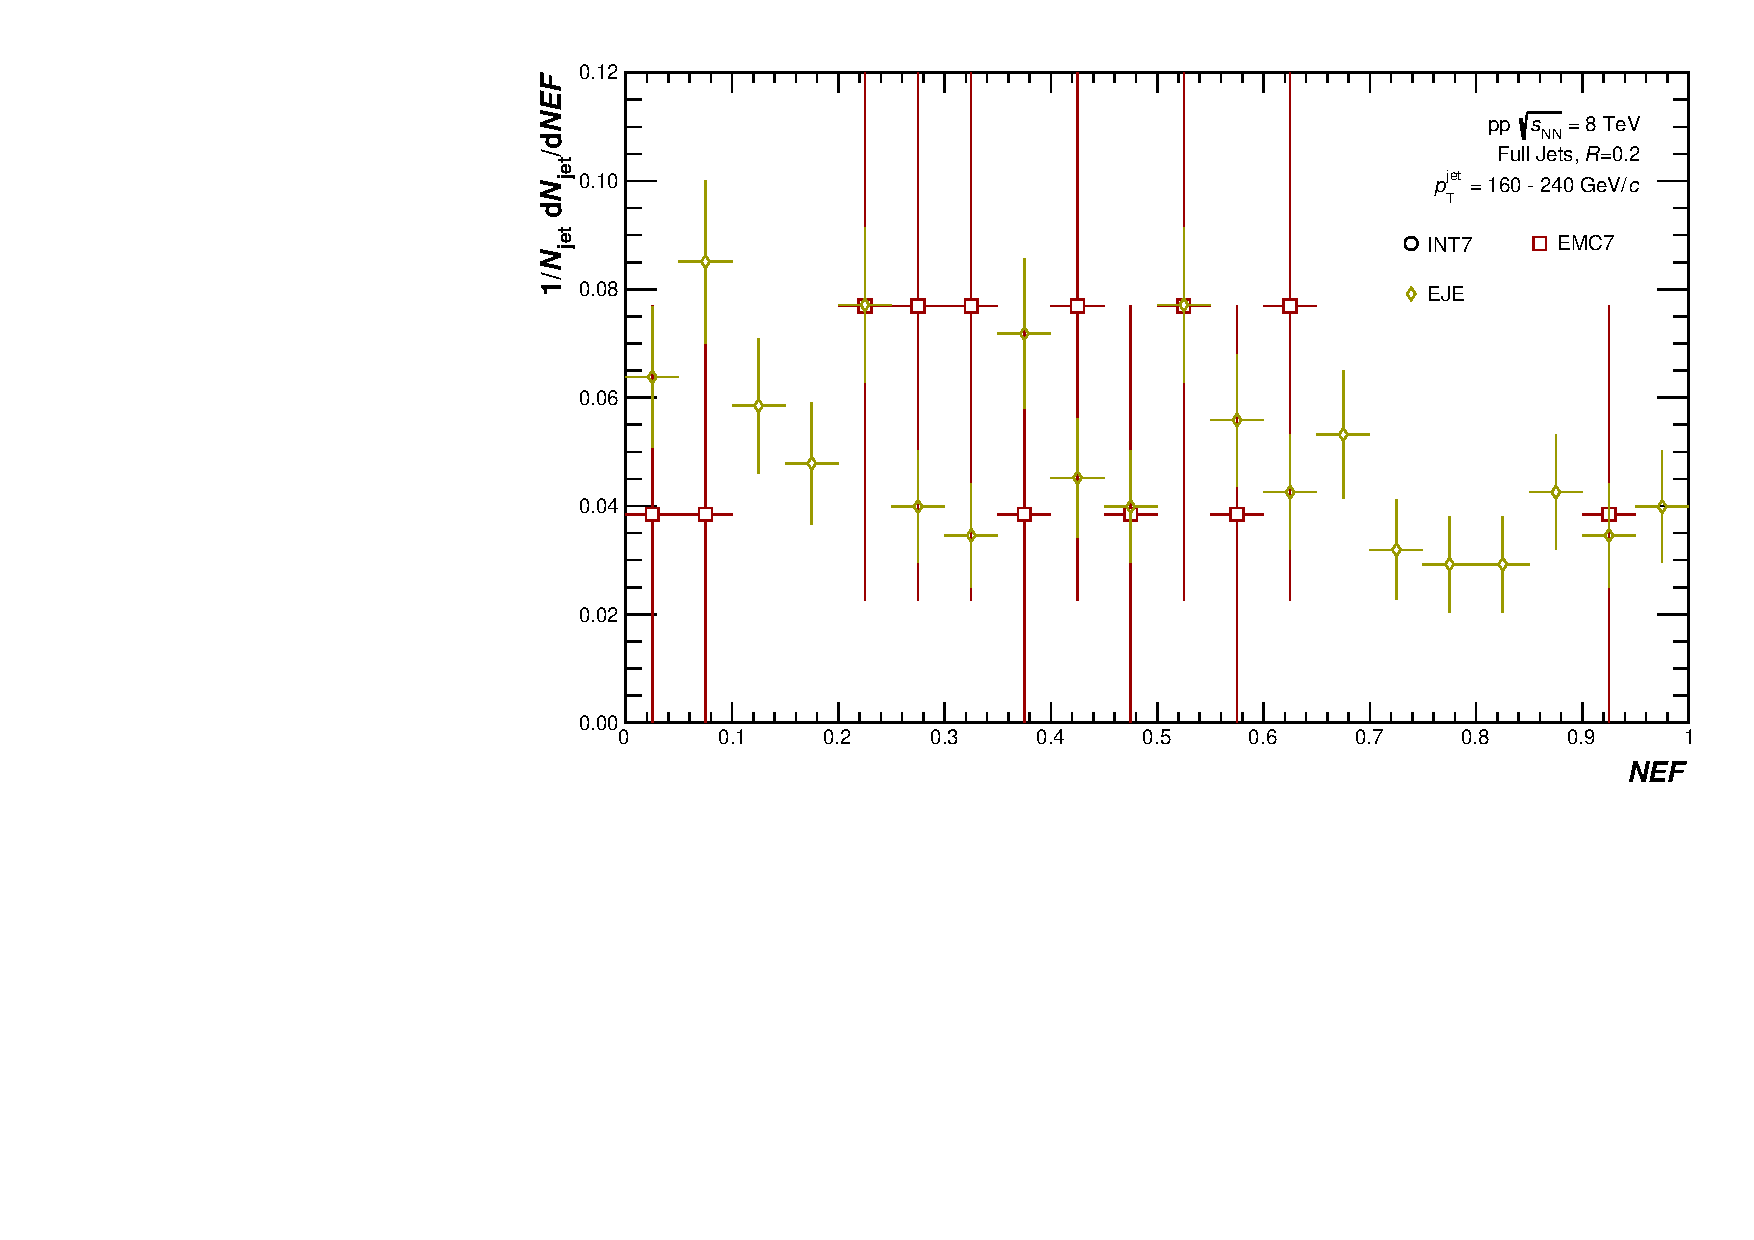
\includegraphics[width=7.5cm]{figures/NEF/All/hNEF_160-240GeV_R02.pdf}
        \vfill\null
        \columnbreak
            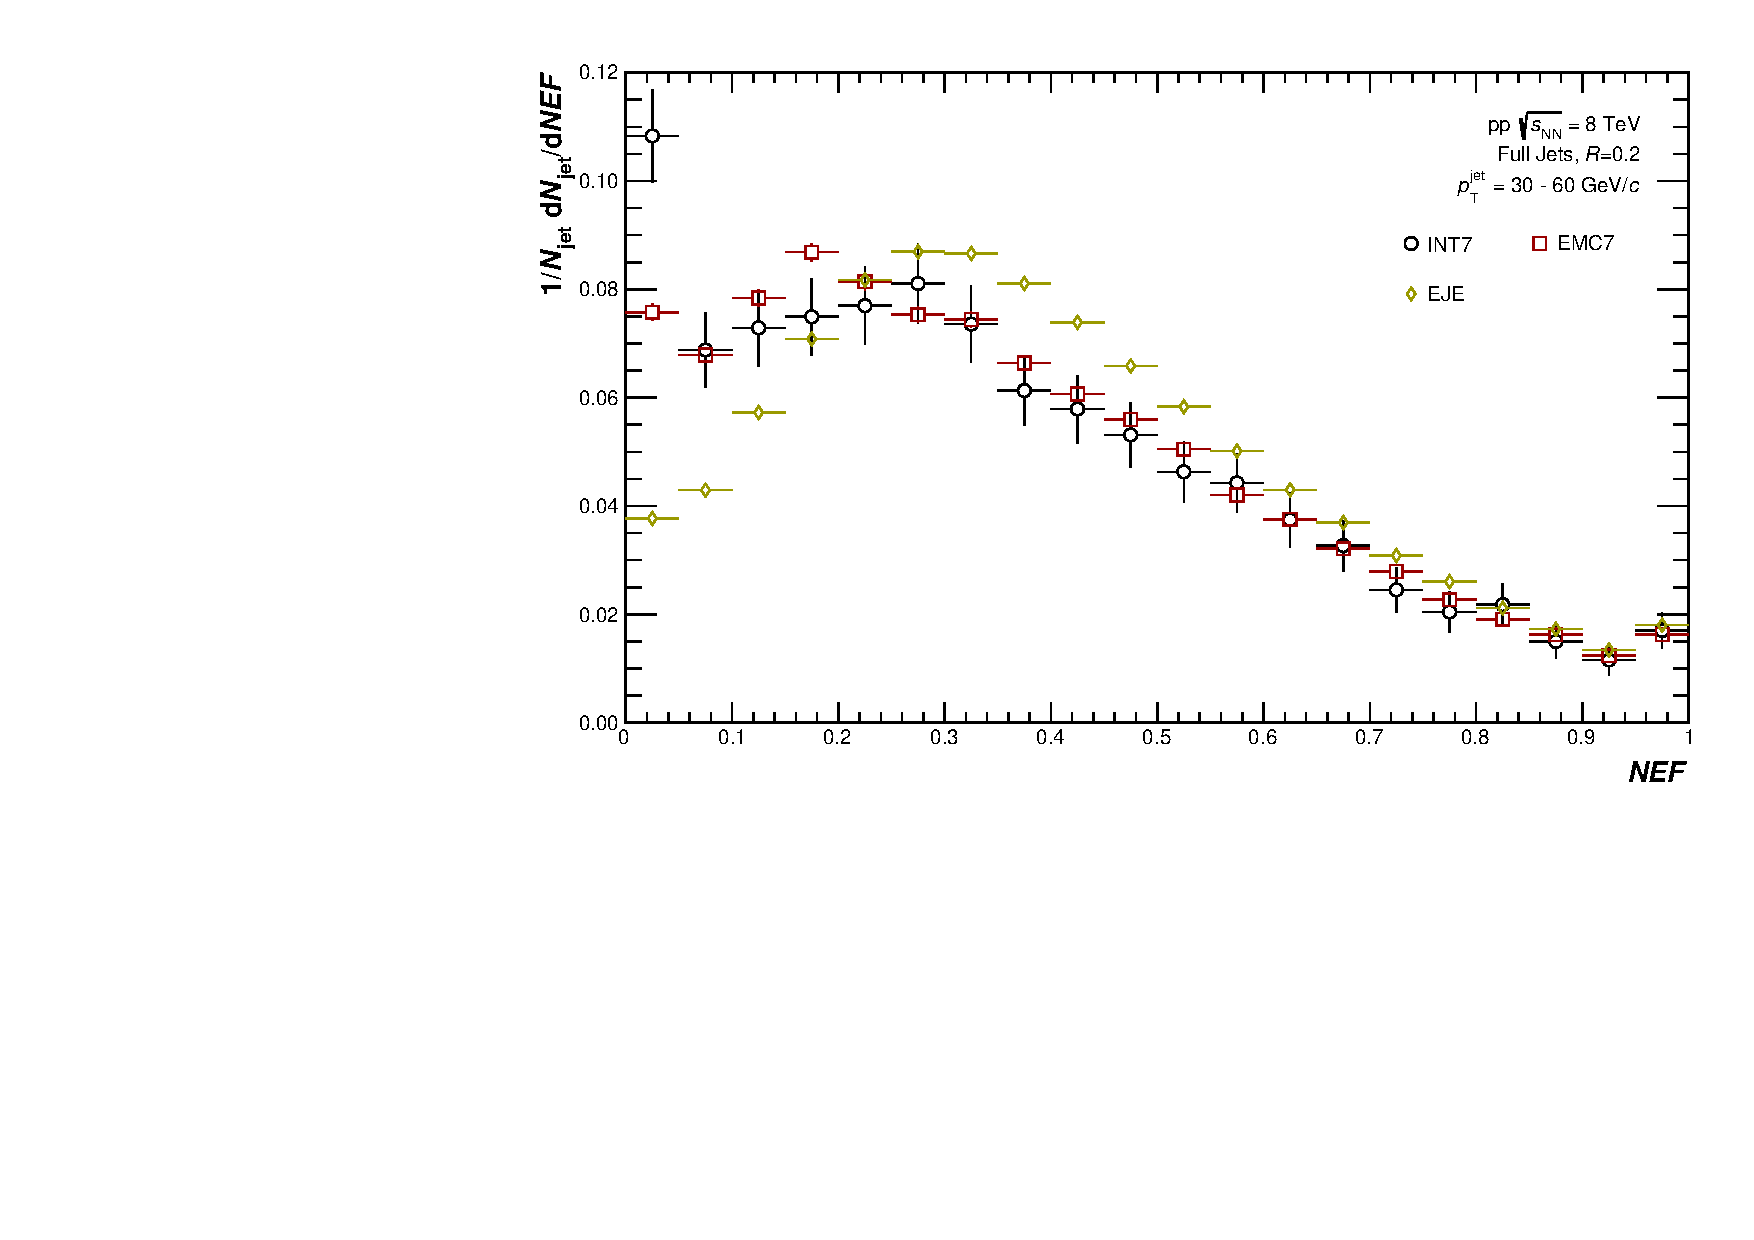
\includegraphics[width=7.5cm]{figures/NEF/All/hNEF_30-60GeV_R02.pdf}
            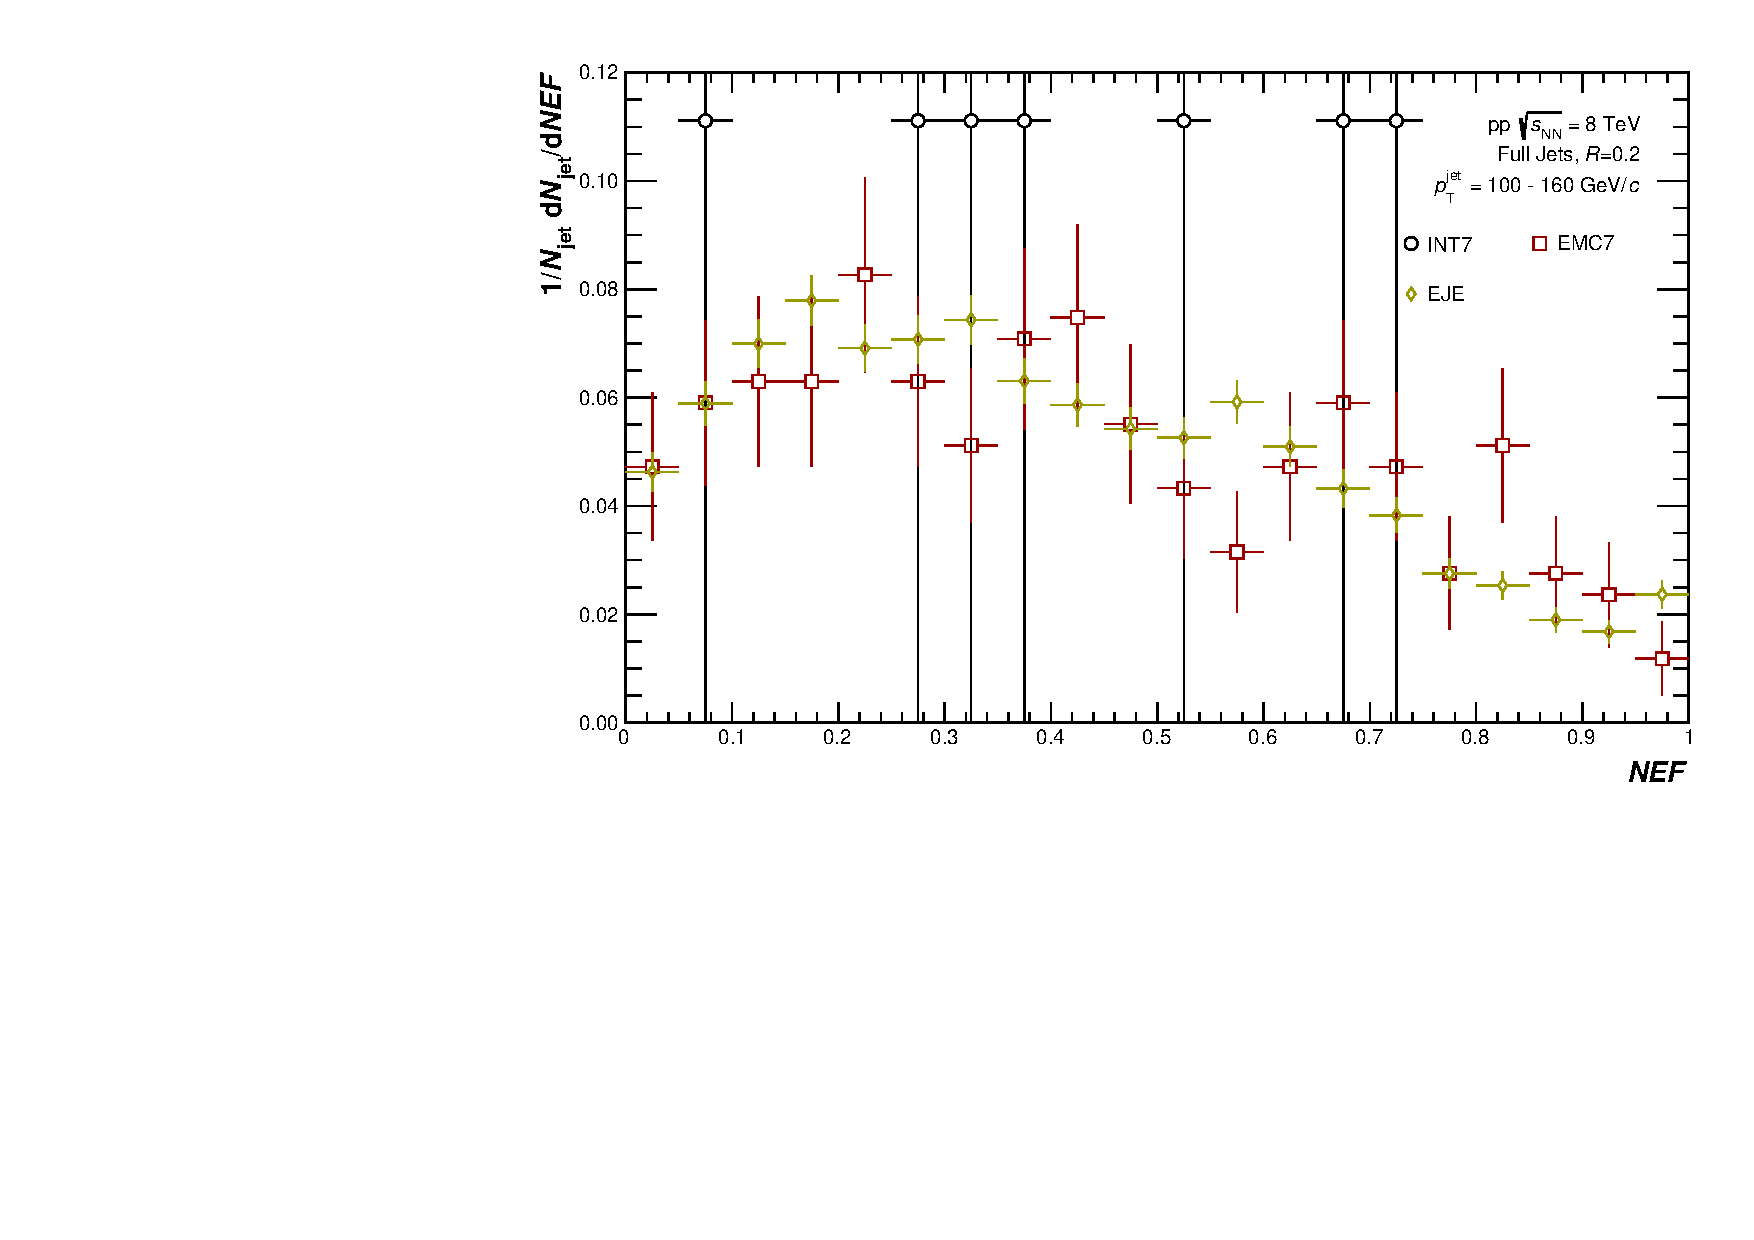
\includegraphics[width=7.5cm]{figures/NEF/All/hNEF_100-160GeV_R02.pdf}
        \vfill\null
    \end{multicols}
    \caption{Neutral energy fraction for jets in \pp collisions found using the minimum bias and EMCal triggers for different bins in jet energy using R = 0.2 jets.}
    \label{fig:NEF}
\end{figure}

\begin{figure}[h!]
    \centering
    \begin{multicols}{2}
            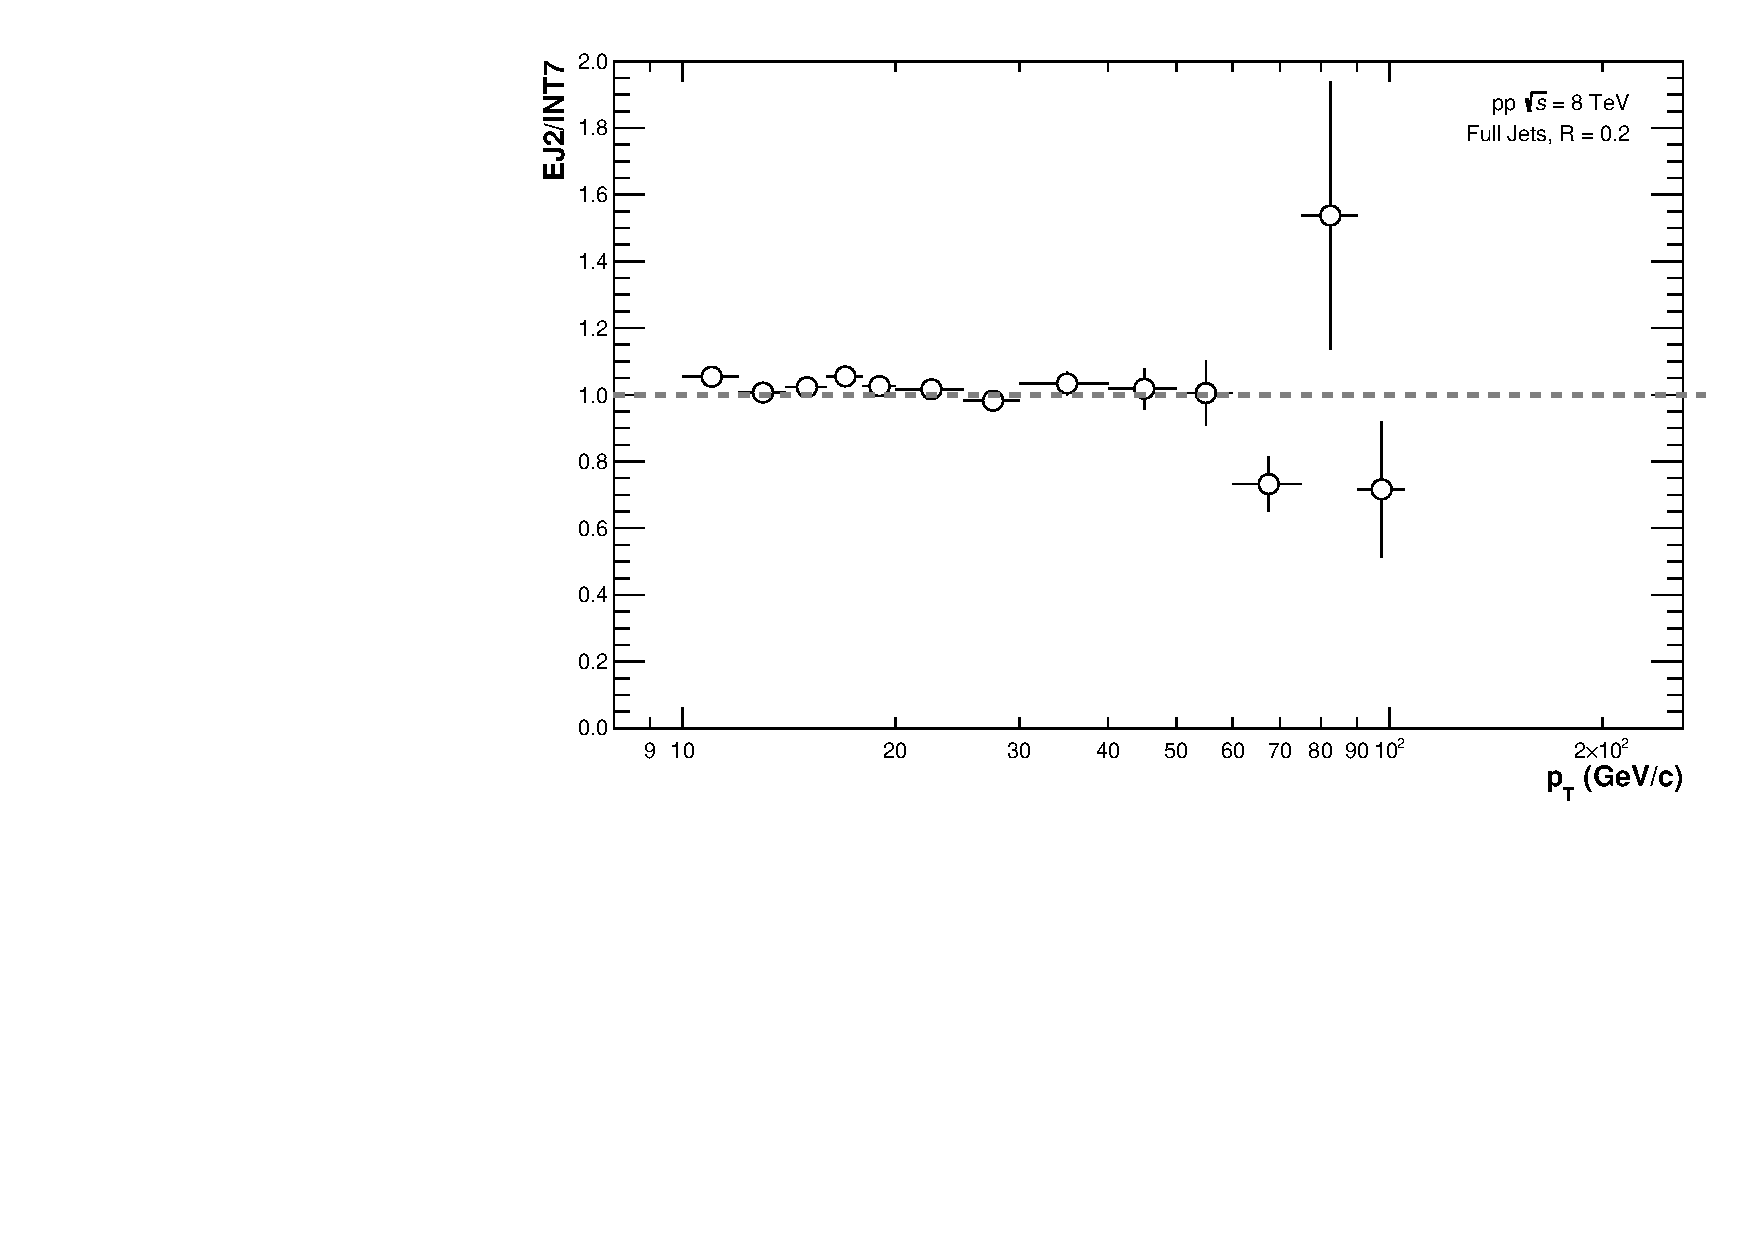
\includegraphics[width=7.5cm]{figures/TriggerSwap/ratio_EMCINT_data_R02.pdf}
        \vfill\null 
        \columnbreak
            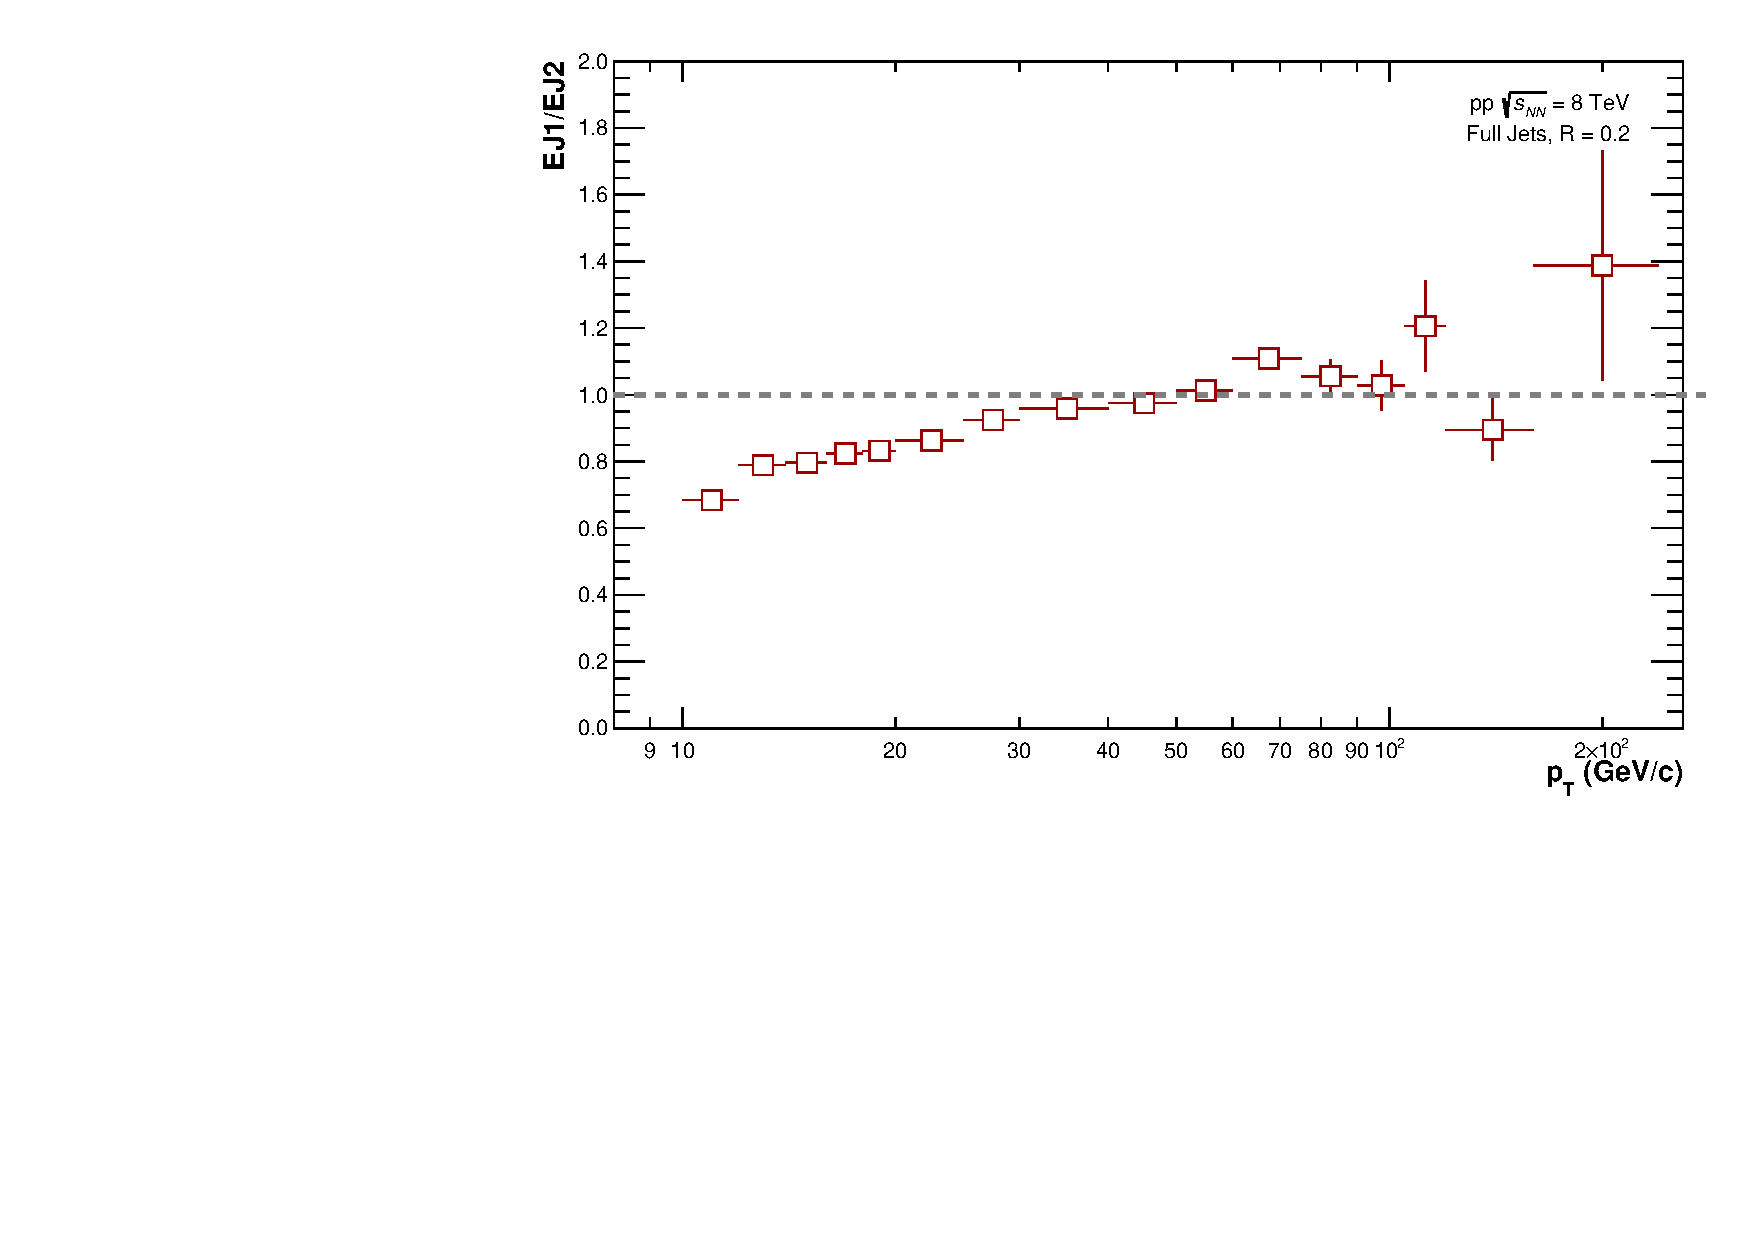
\includegraphics[width=7.5cm]{figures/TriggerSwap/ratio_EJEEMC_data_R02.pdf}
        \vfill\null
    \end{multicols}
    \caption{Ratios in \pp data of EMC7/INT7 triggers (left) and EJE/EMC7 triggers (right).}
    \label{fig:trigger_ratios}
\end{figure}

As the trigger selects jets based on its neutral energy component, it introduces a bias on the selected jets that vanishes only at higher \pT. Fig. \ref{fig:NEF} shows the comparison of the distribution of the neutral energy fraction (NEF) of \pp jets in min. bias and triggered events for various bins in \pT for R = 0.2 jets. For other radii and equivalent plots in \pPb, see appendix \ref{sec:appendixTriggerBiaspPb}. The NEF is the fraction of the total energy of the track + EMCal cluster that comes from the neutral component. At lower \pT, the distribution in EMCal triggered events is shifted towards higher NEF values, since for jets close to the threshold, the dominant part of the energy must originate from neutral particles in order to fire the trigger. Only for jets with \pT larger than 30 (60) GeV/c, the distributions for the EMC7 (EJE) trigger start overlapping with the distribution in minimum bias events (for \pPb, this occurs at 30 (50) GeV for the EJ2 (EJ1) trigger). Additionally, at lower \pT, an effect can be seen from the different track and cluster \pT cutoffs (150 MeV for tracks, 300 MeV for clusters). As jet \pT decreases, it is more likely to find tracks than clusters, since the cutoff for tracks is lower. As jet \pT increases, the distributions begin to overlap. This is apparent in the 30-60 GeV/c region, but minimum bias statistics are too small to see beyond this \pT region. This effect can also be seen in figure 100 of the 2022 EMCal Performance paper \cite{EMCalPerformance}. Fig. \ref{fig:trigger_ratios} shows the \pT dependence of the jet yield ratio of trigger/min bias, which rises with \pT until a plateau is reached at 30 (60) GeV. At this point, the trigger is fully efficient, and the bias vanishes. For the analysis, jets are selected in triggered events only in the region where the trigger is bias-free. This will be discussed further in section \ref{sec:triggerCorrection}.

The trigger response in simulations is obtained by applying the same sliding window algorithm as implemented in the trigger hardware. A single EMCal FEE card provides readout for 32 towers, arranged in an 8x4 configuration. A FastOR covers a 2x2 tower group, and can cross boundaries between FEE cards. It provides a fast way to determine whether the 2x2 group is above a given threshold, as well as a rough energy reading. The trigger patches are calculated based on the energy from overlapping 4x4 tower sums that come from the FEE (Front End Electronics) simulation summed to FastORs. As the energy measurements in the trigger hardware suffer from residual decalibration, the energy is smeared based on the correlation between the energy measured in the FastOR and the calibrated FEE energy obtained from data. Realistic acceptance is simulated by removing FastOR energies based on the trigger mask in data. Triggered events are required to have at least one trigger patch above the nominal threshold. The description of the trigger bias in simulation is tested comparing the distributions of neutral energy fraction, z$_{ch}$, and z$_{neutral}$ between data and simulation. The objects z$_{ch}$ and z$_{neutral}$ are the fraction of the jet \pT coming from charged and neutral particles, respectively. Fig. \ref{fig:TriggerBiasNEFR02} shows the comparison of the neutral energy fraction for jets from \pp collisions with R=0.2 in triggered events between data and simulations for different bins in \pT (for other radii and the comparison of z$_{ch}$ and z$_{neutral}$, see appendix \ref{sec:appendixTriggerBiasRatios}). For the equivalent plots in \pPb, see appendix \ref{sec:appendixTriggerBiasRatiospPb}. The distributions obtained from simulation are in good agreement with the distributions obtained from data. 

Fig. \ref{fig:TriggerEfficiency} shows the trigger efficiency for jets with R=0.2 - R=0.6, obtained from taking the ratio of trigger/min. bias in simulations. The trigger gets adequately efficient at a jet \pT of 60 (30) GeV/c for the EJE (EMC7) trigger. In the low energy region, other detector effects which are not simulated (i.e. random noise) play a role. The simulated trigger efficiency will overpredict the correction, and thus the Monte-Carlo based correction can be trusted only in the higher-pt region of the turn-on.

\begin{figure}[h!]
    \centering
    \begin{multicols}{2}
            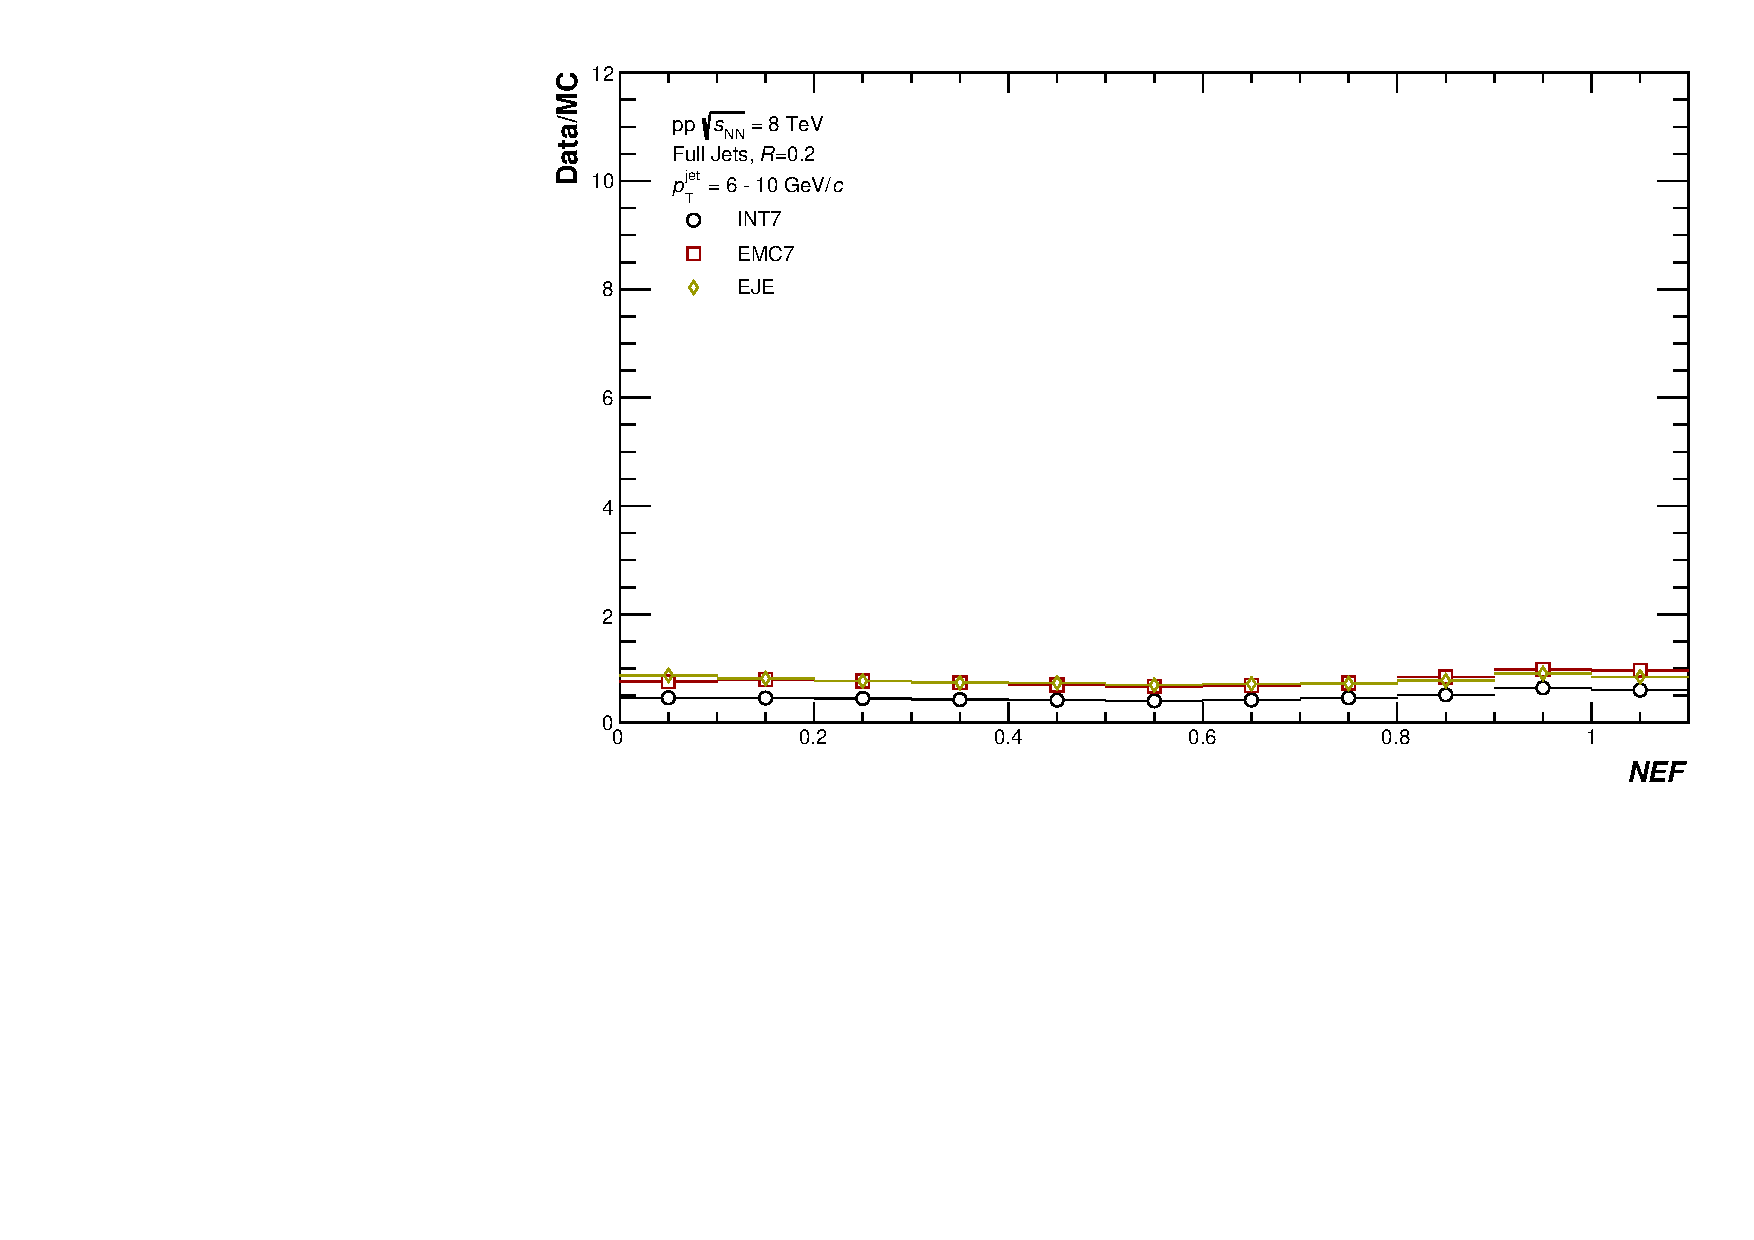
\includegraphics[width=7.5cm]{figures/TriggerBias/NEF/hNEF_ptBin0_R02.pdf}
            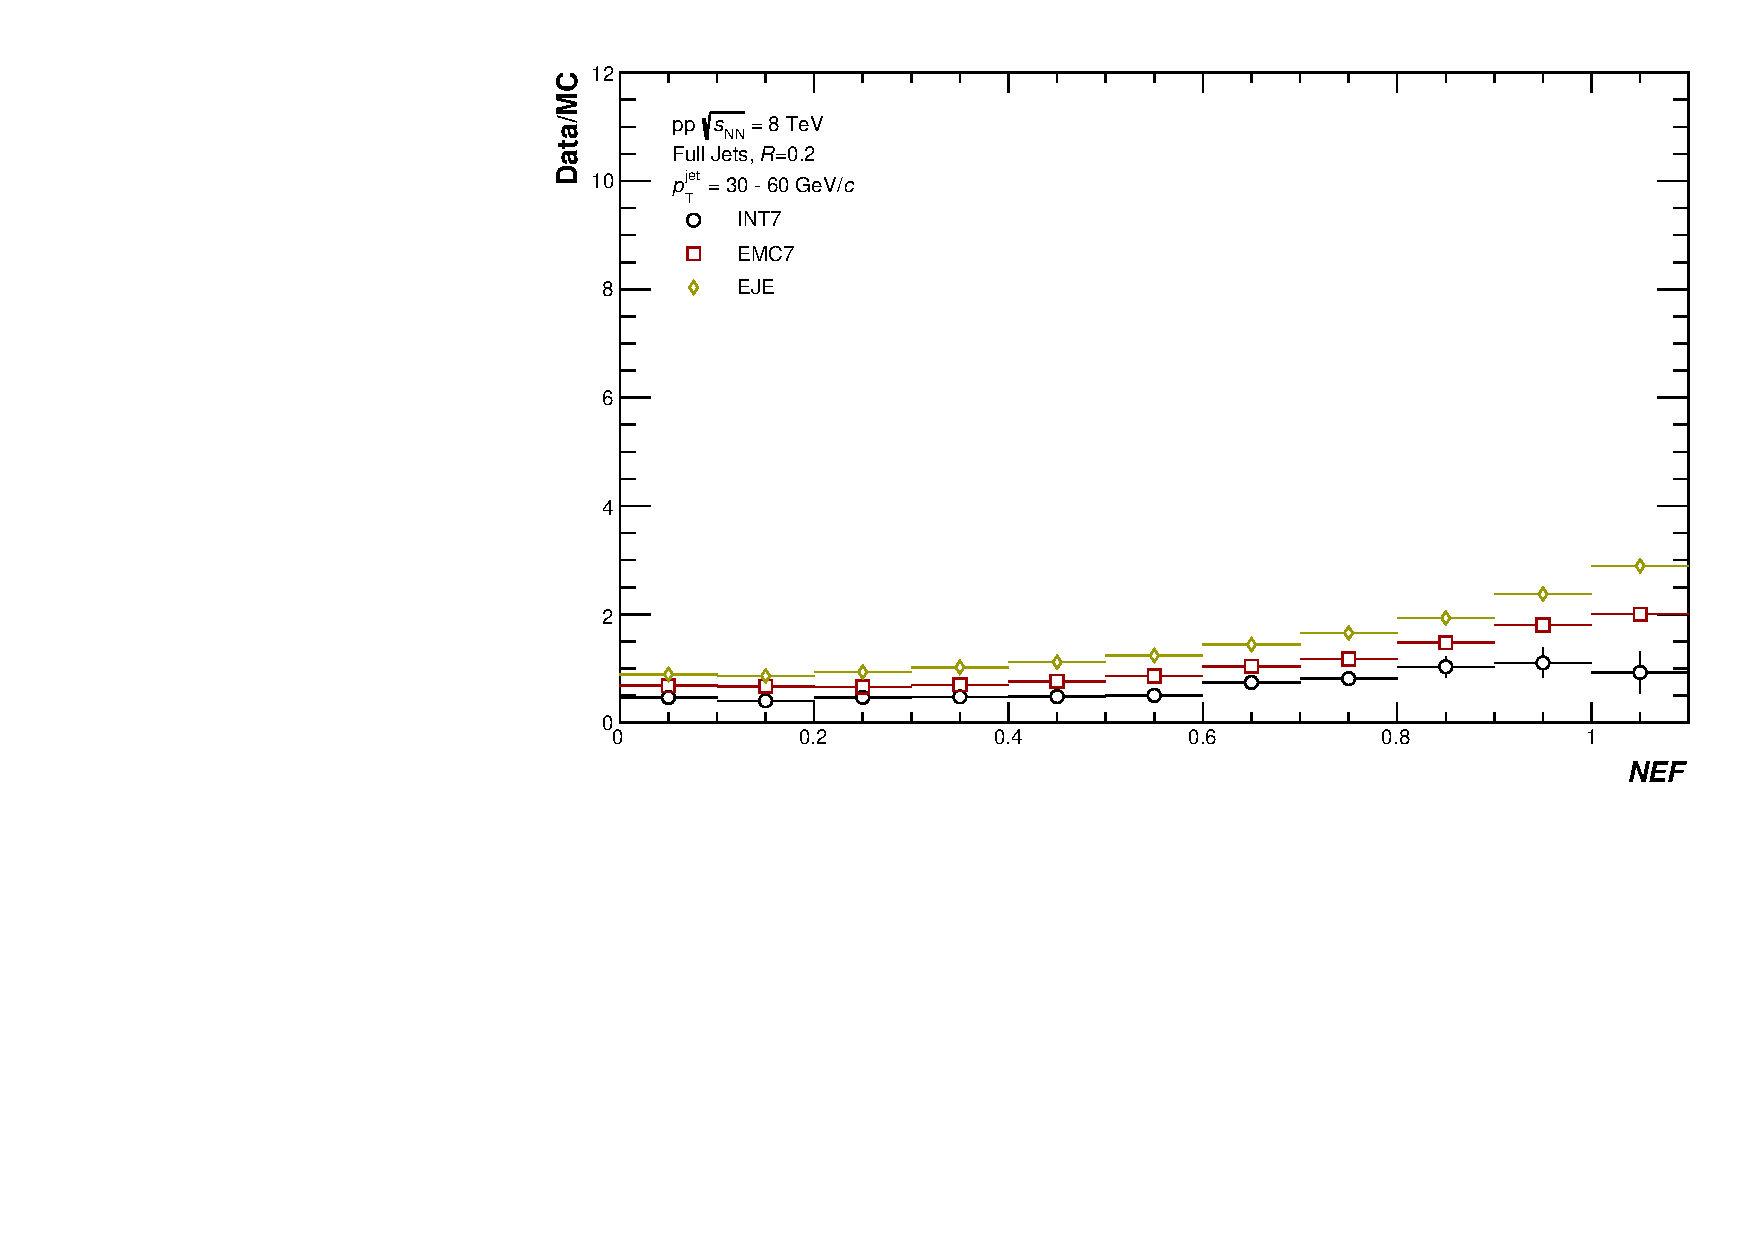
\includegraphics[width=7.5cm]{figures/TriggerBias/NEF/hNEF_ptBin2_R02.pdf}
            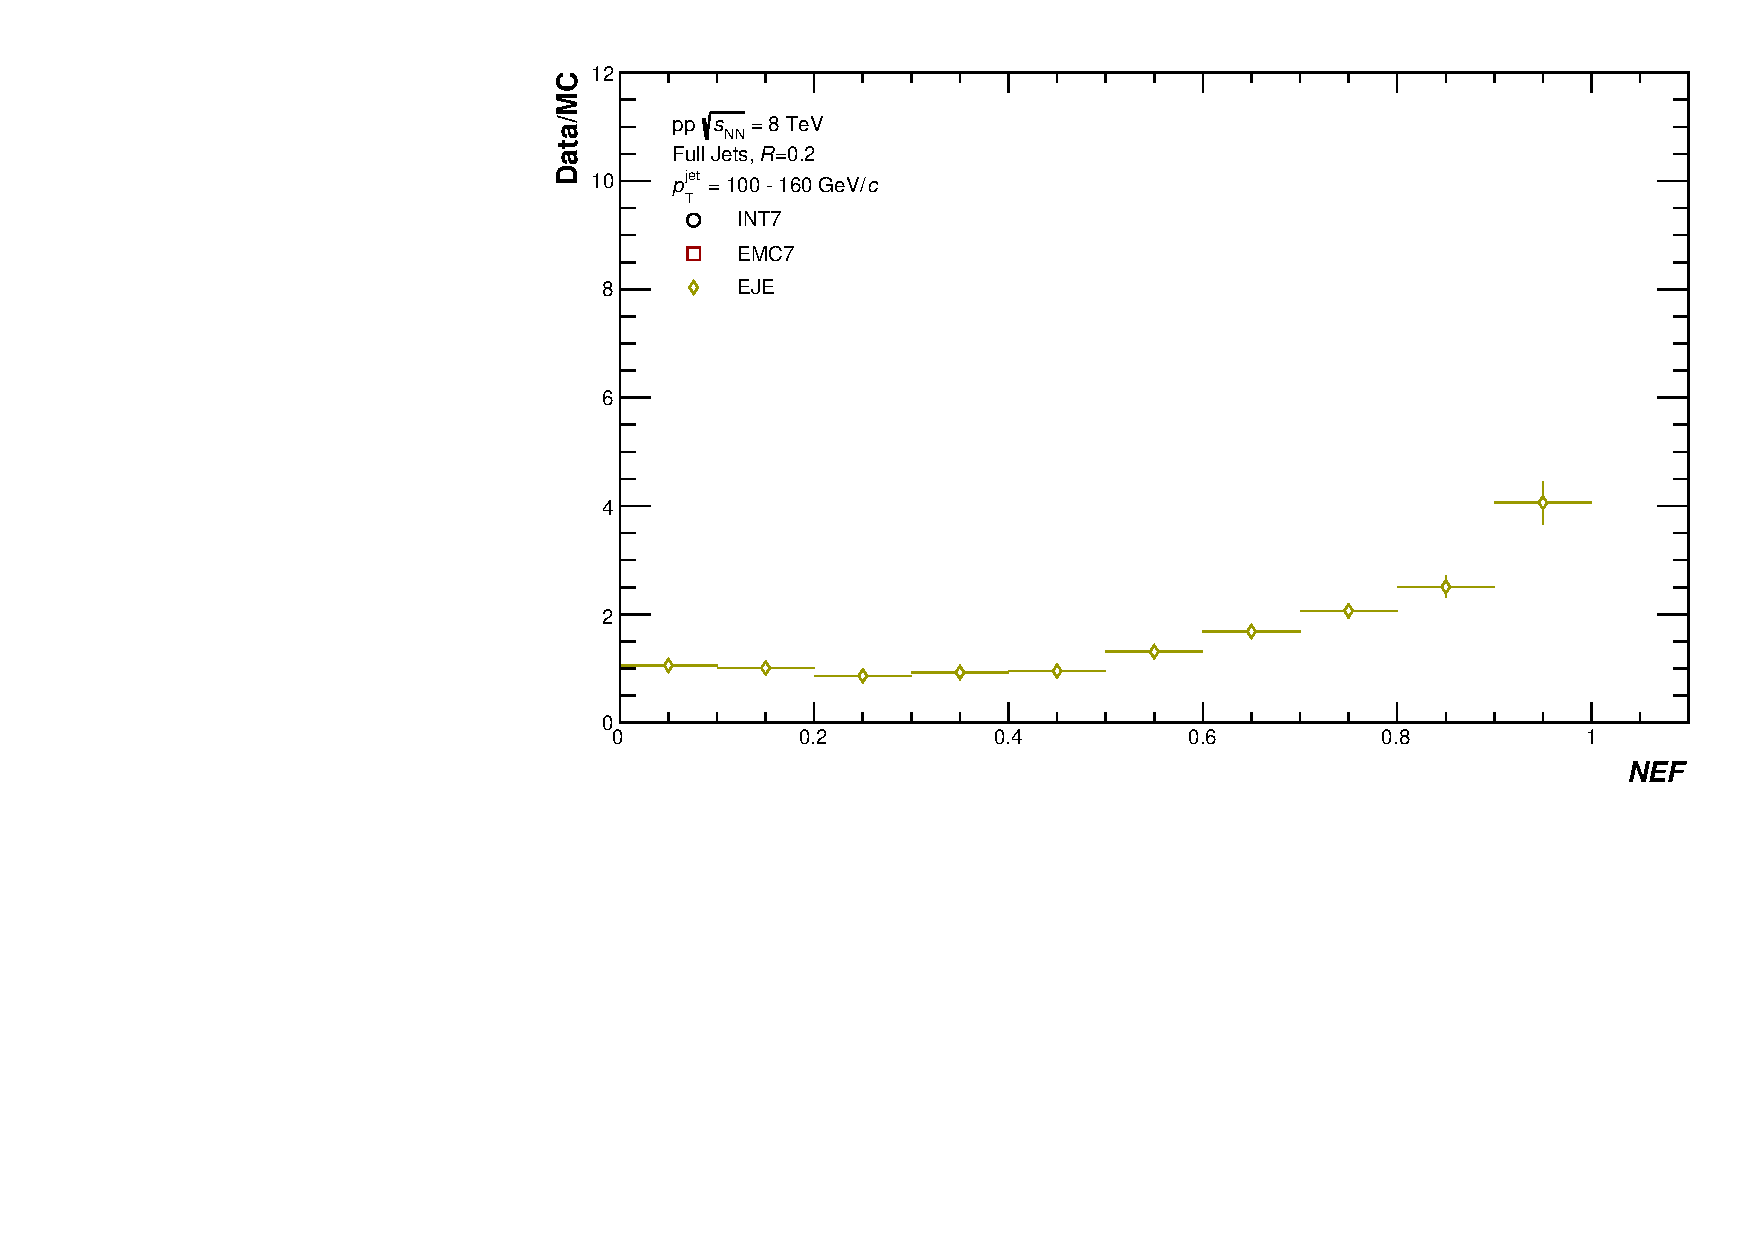
\includegraphics[width=7.5cm]{figures/TriggerBias/NEF/hNEF_ptBin4_R02.pdf}
        \vfill\null
        \columnbreak
            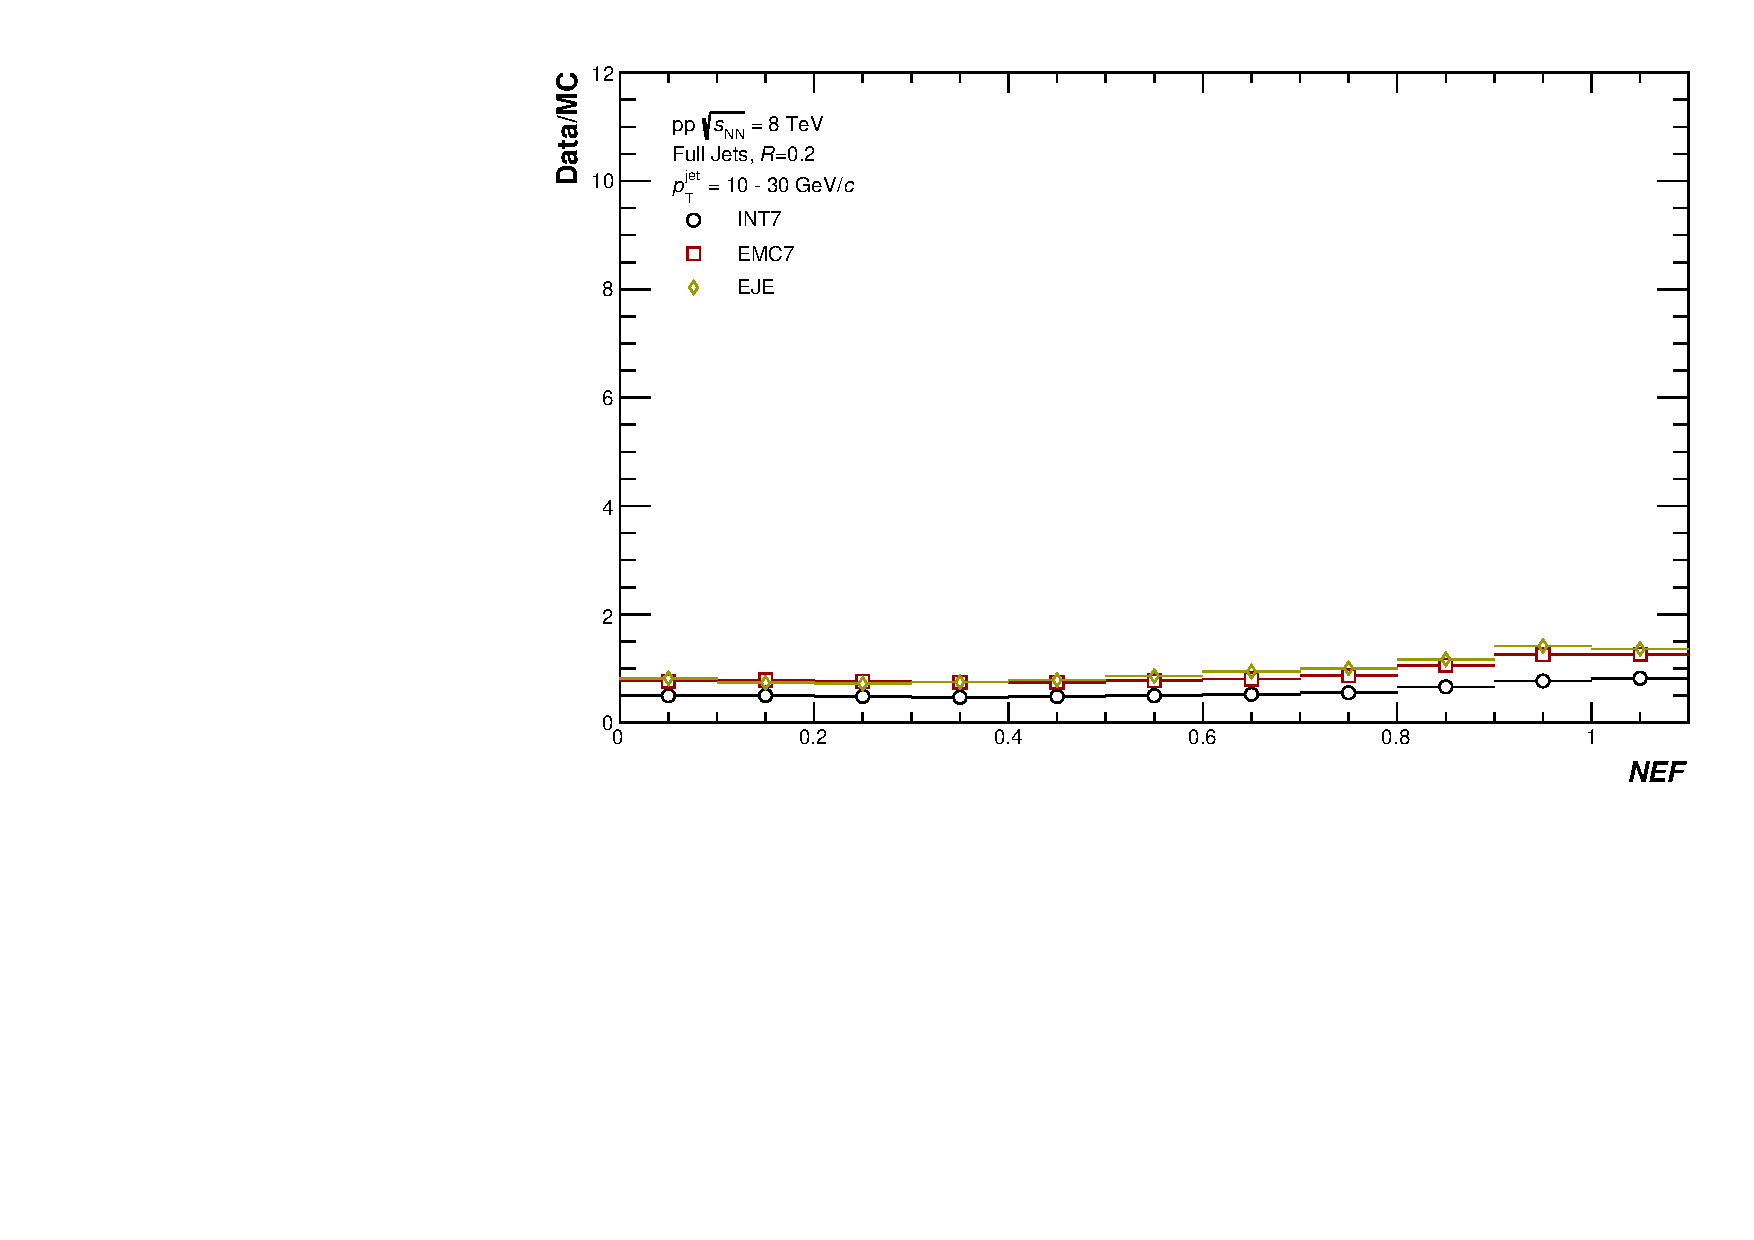
\includegraphics[width=7.5cm]{figures/TriggerBias/NEF/hNEF_ptBin1_R02.pdf}
            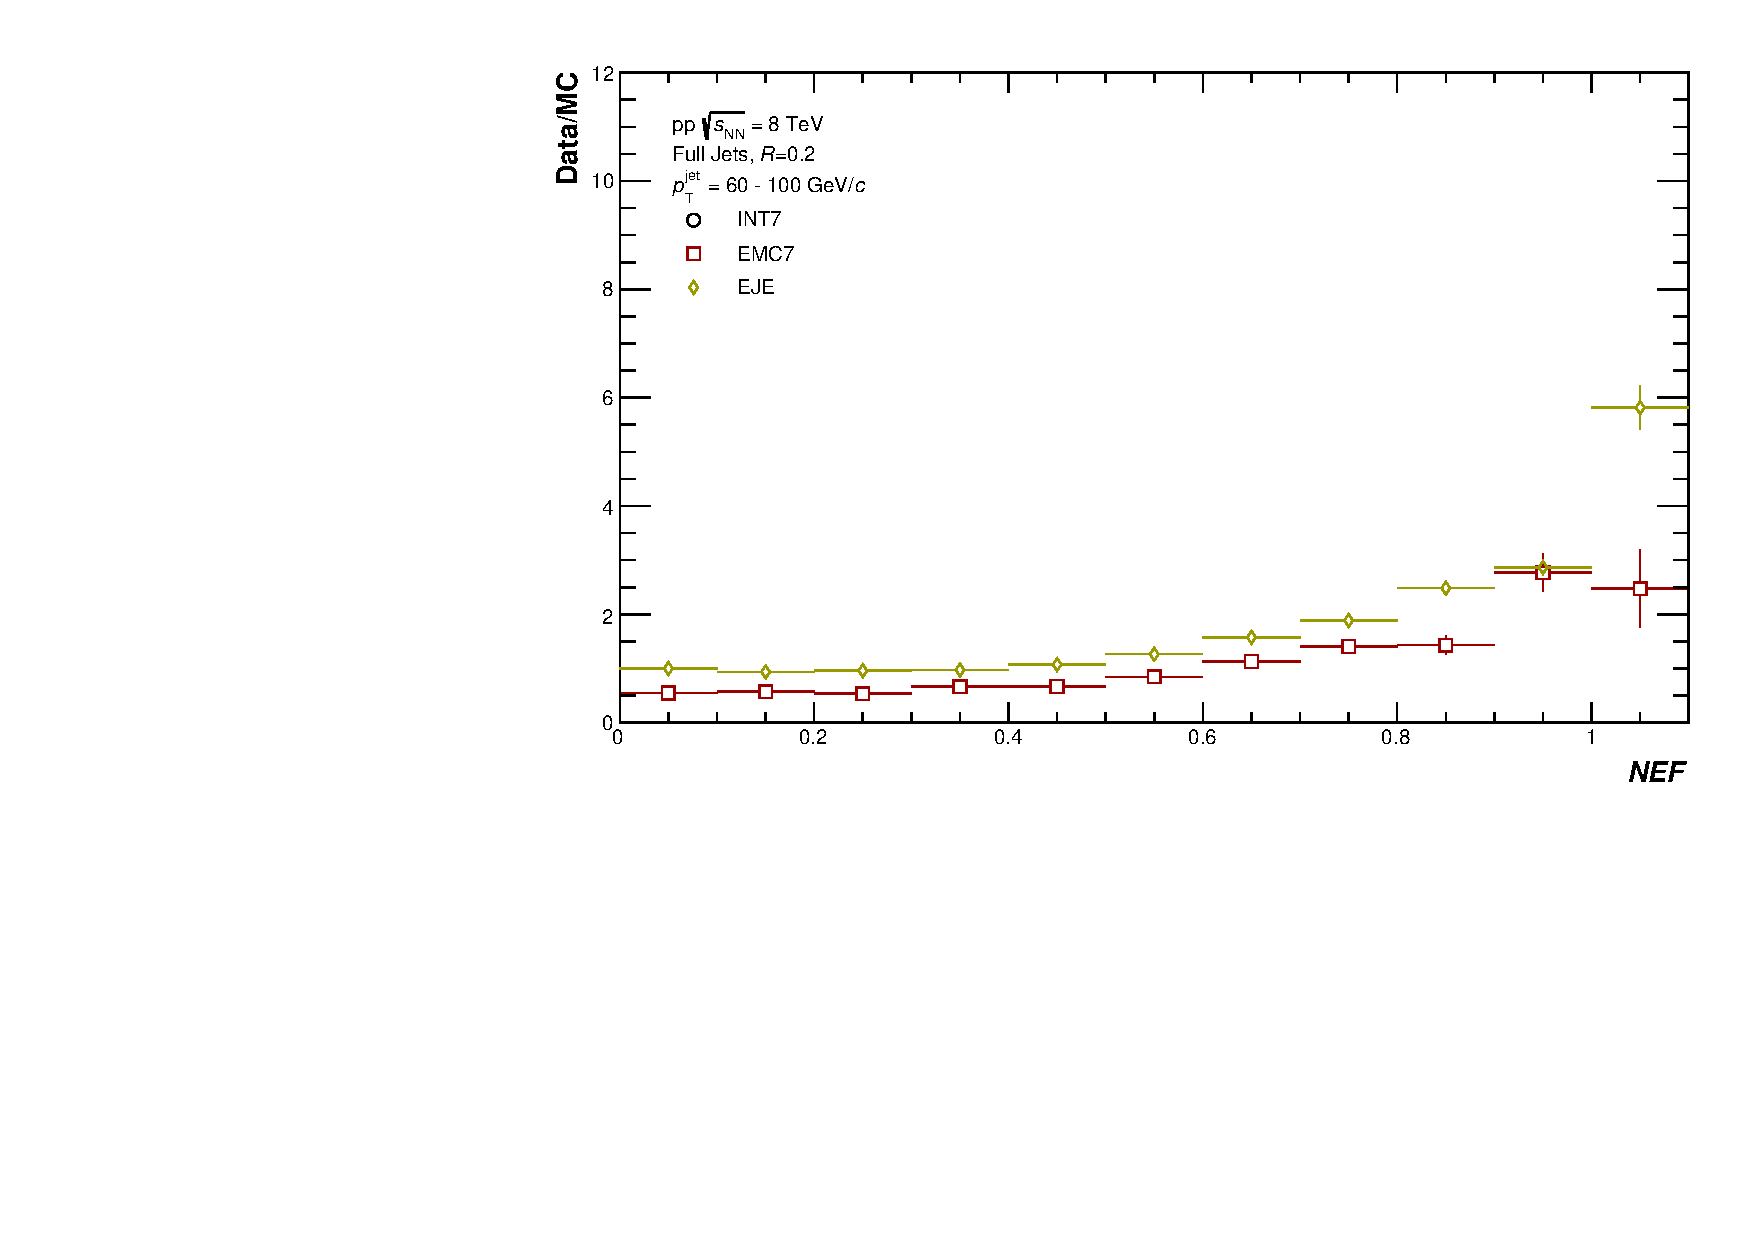
\includegraphics[width=7.5cm]{figures/TriggerBias/NEF/hNEF_ptBin3_R02.pdf}
            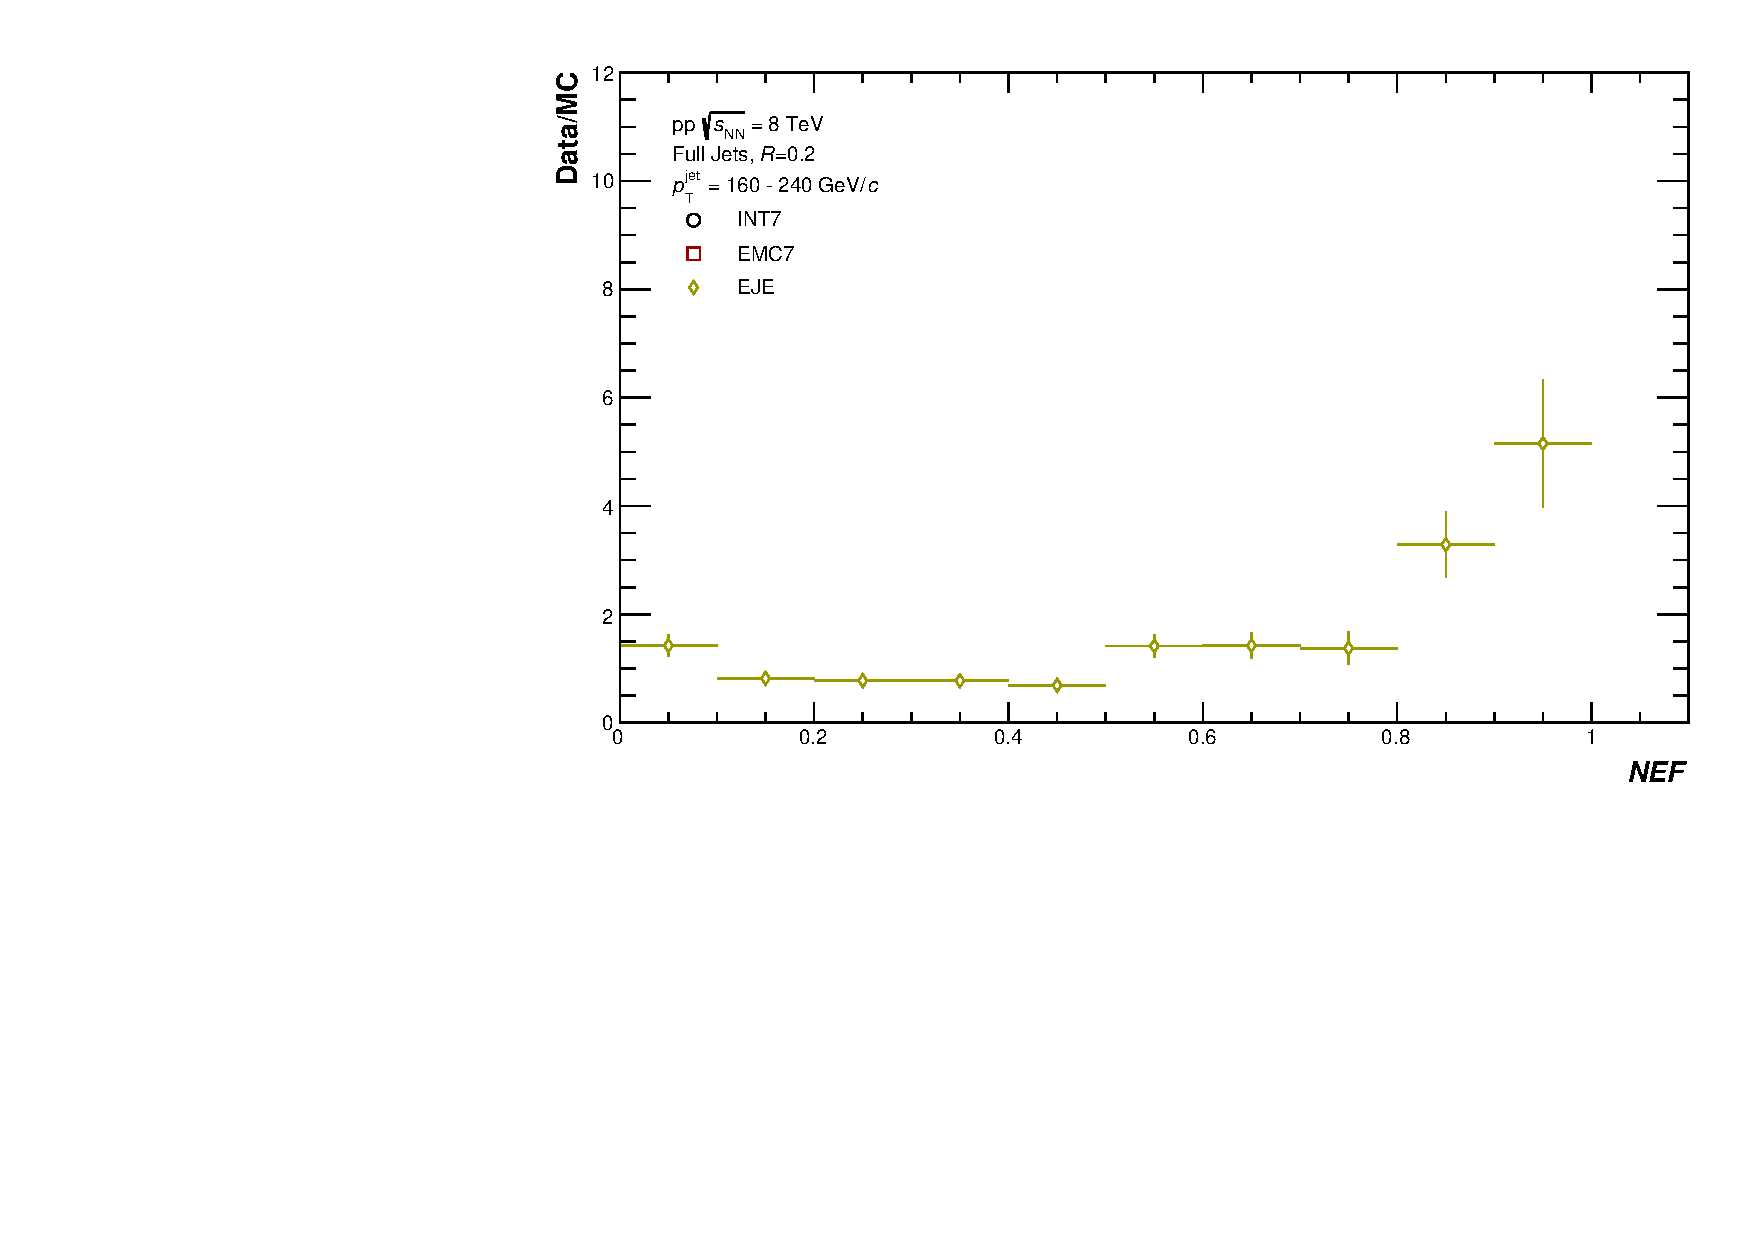
\includegraphics[width=7.5cm]{figures/TriggerBias/NEF/hNEF_ptBin5_R02.pdf}
        \vfill\null
    \end{multicols}
    \caption{NEF ratios of \pp data to MC for different bins in jet \pT and a jet radius of R=0.2.}
    \label{fig:TriggerBiasNEFR02}
\end{figure}

\begin{figure}[h!]
    \centering
    \begin{multicols}{2}
            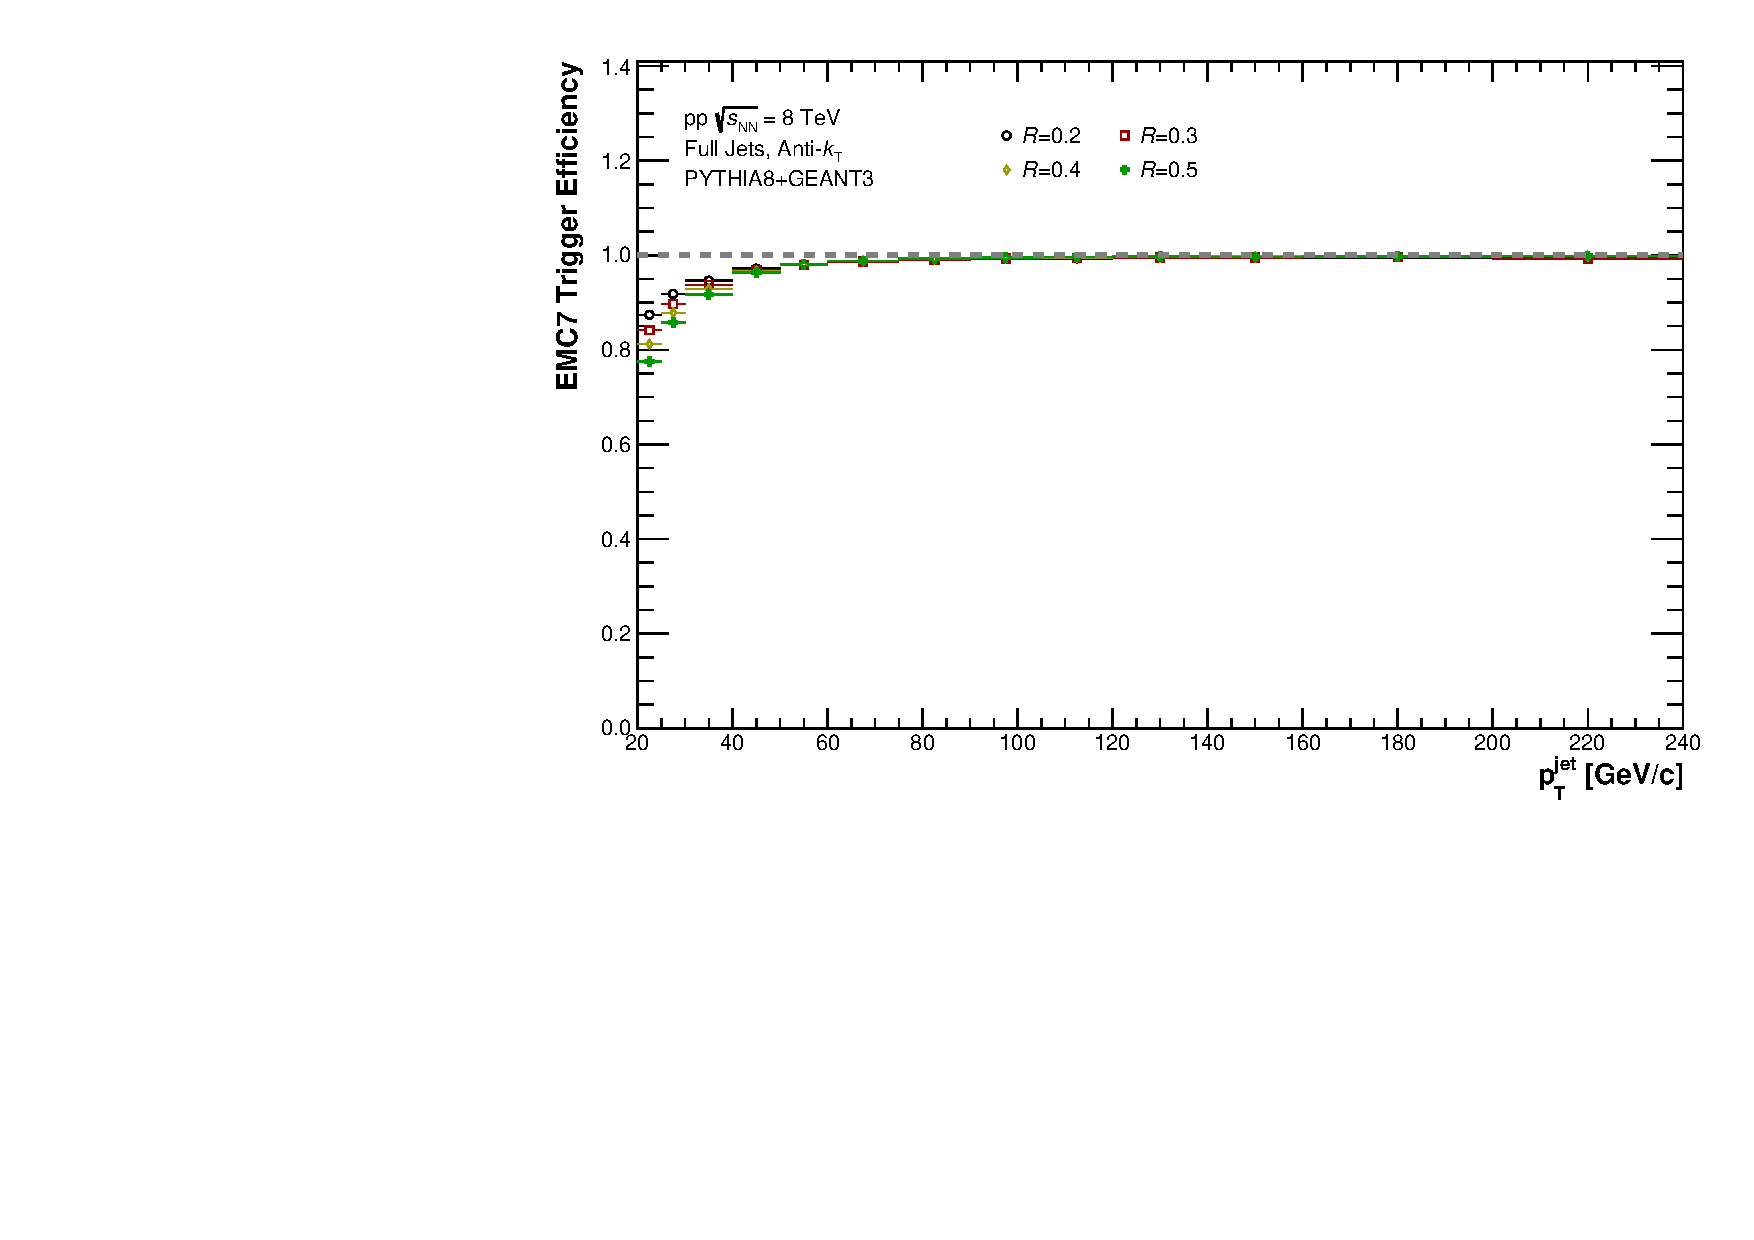
\includegraphics[width=7.5cm]{figures/TriggerEfficiency/hEfficiency_EMC7.pdf}
        \vfill\null
        \columnbreak
            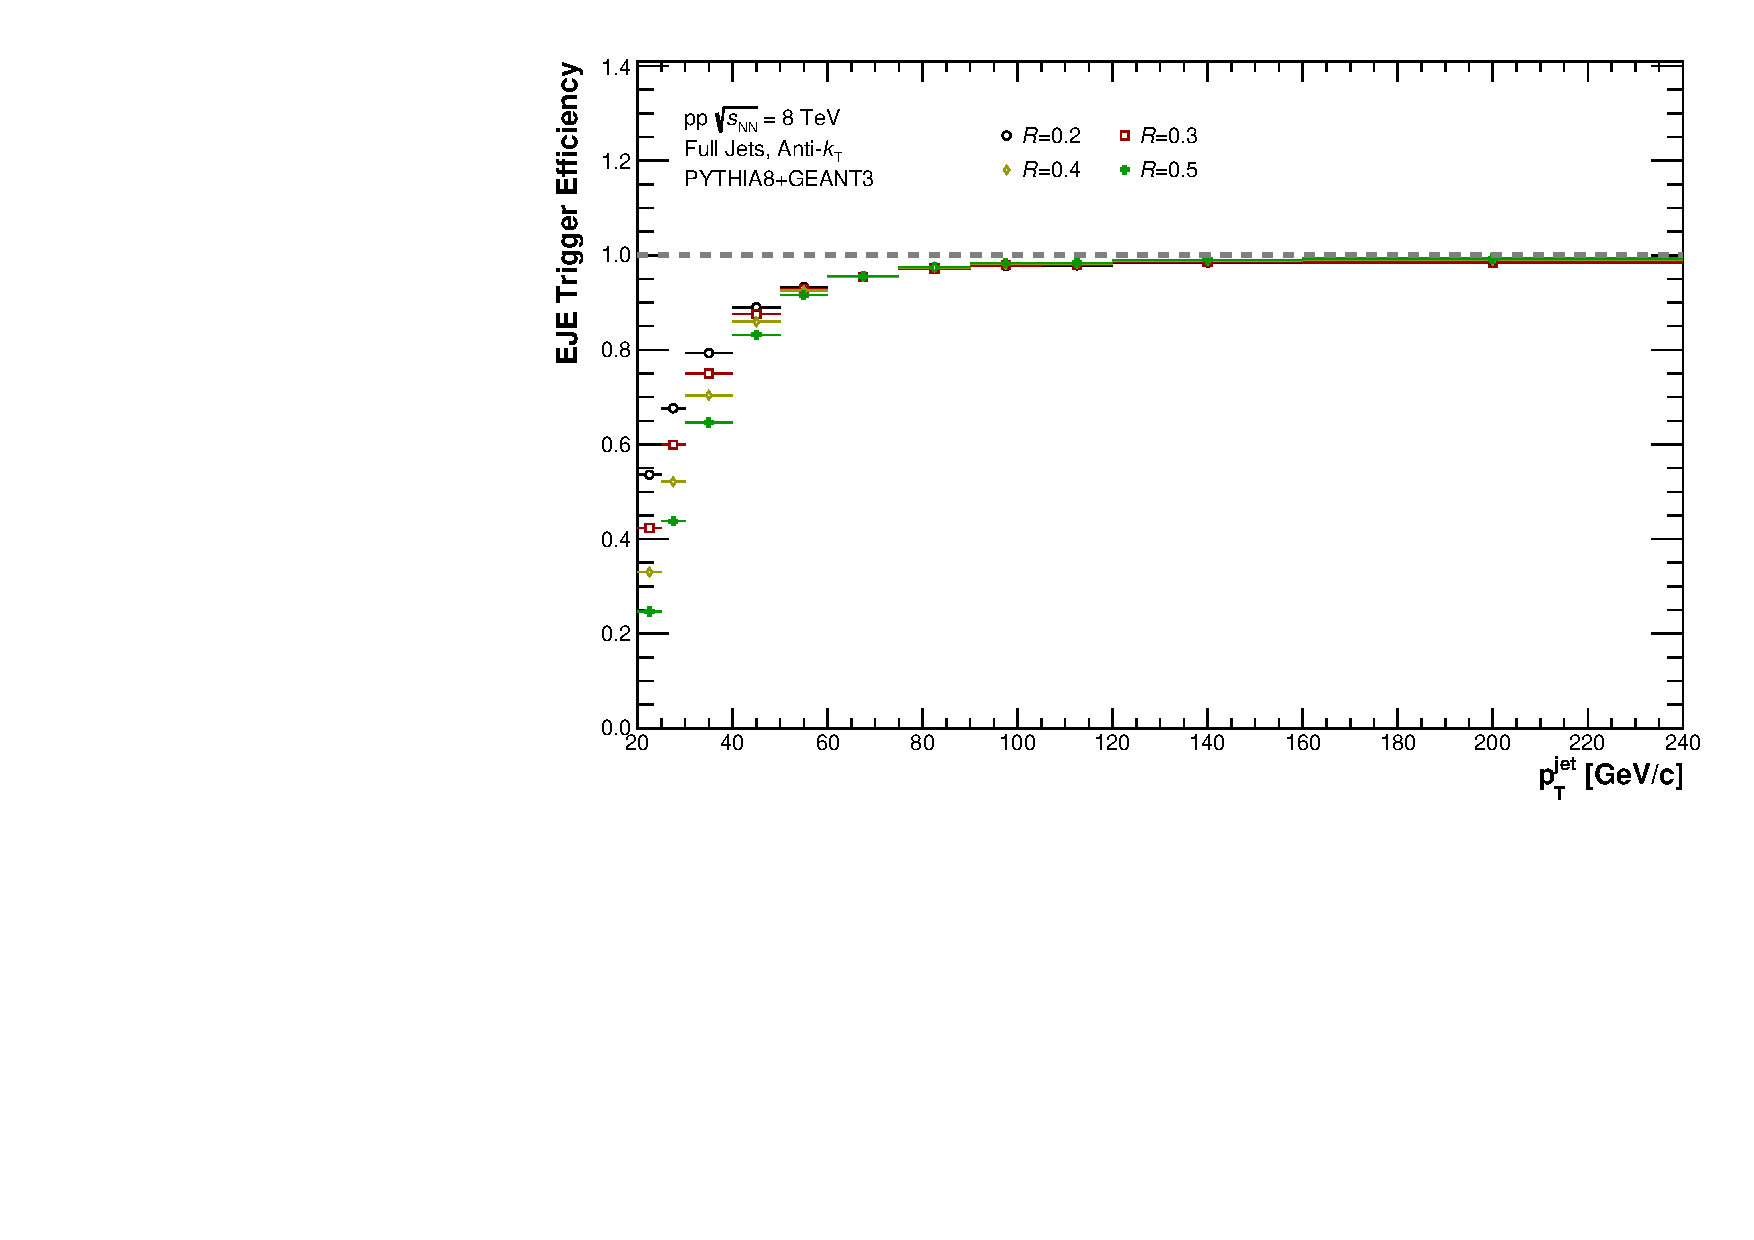
\includegraphics[width=7.5cm]{figures/TriggerEfficiency/hEfficiency_EJE.pdf}
        \vfill\null
    \end{multicols}
    \caption{Trigger efficiency for the EMC7 trigger (left) and the EJE trigger (right), found by taking the ratio of trigger/min bias in \pp simulation.}
    \label{fig:TriggerEfficiency}
\end{figure}

\subsection{Instrumental Response}
\label{sec:InstResponse}

\begin{figure}[h!]
    \centering
    \begin{multicols}{2}
            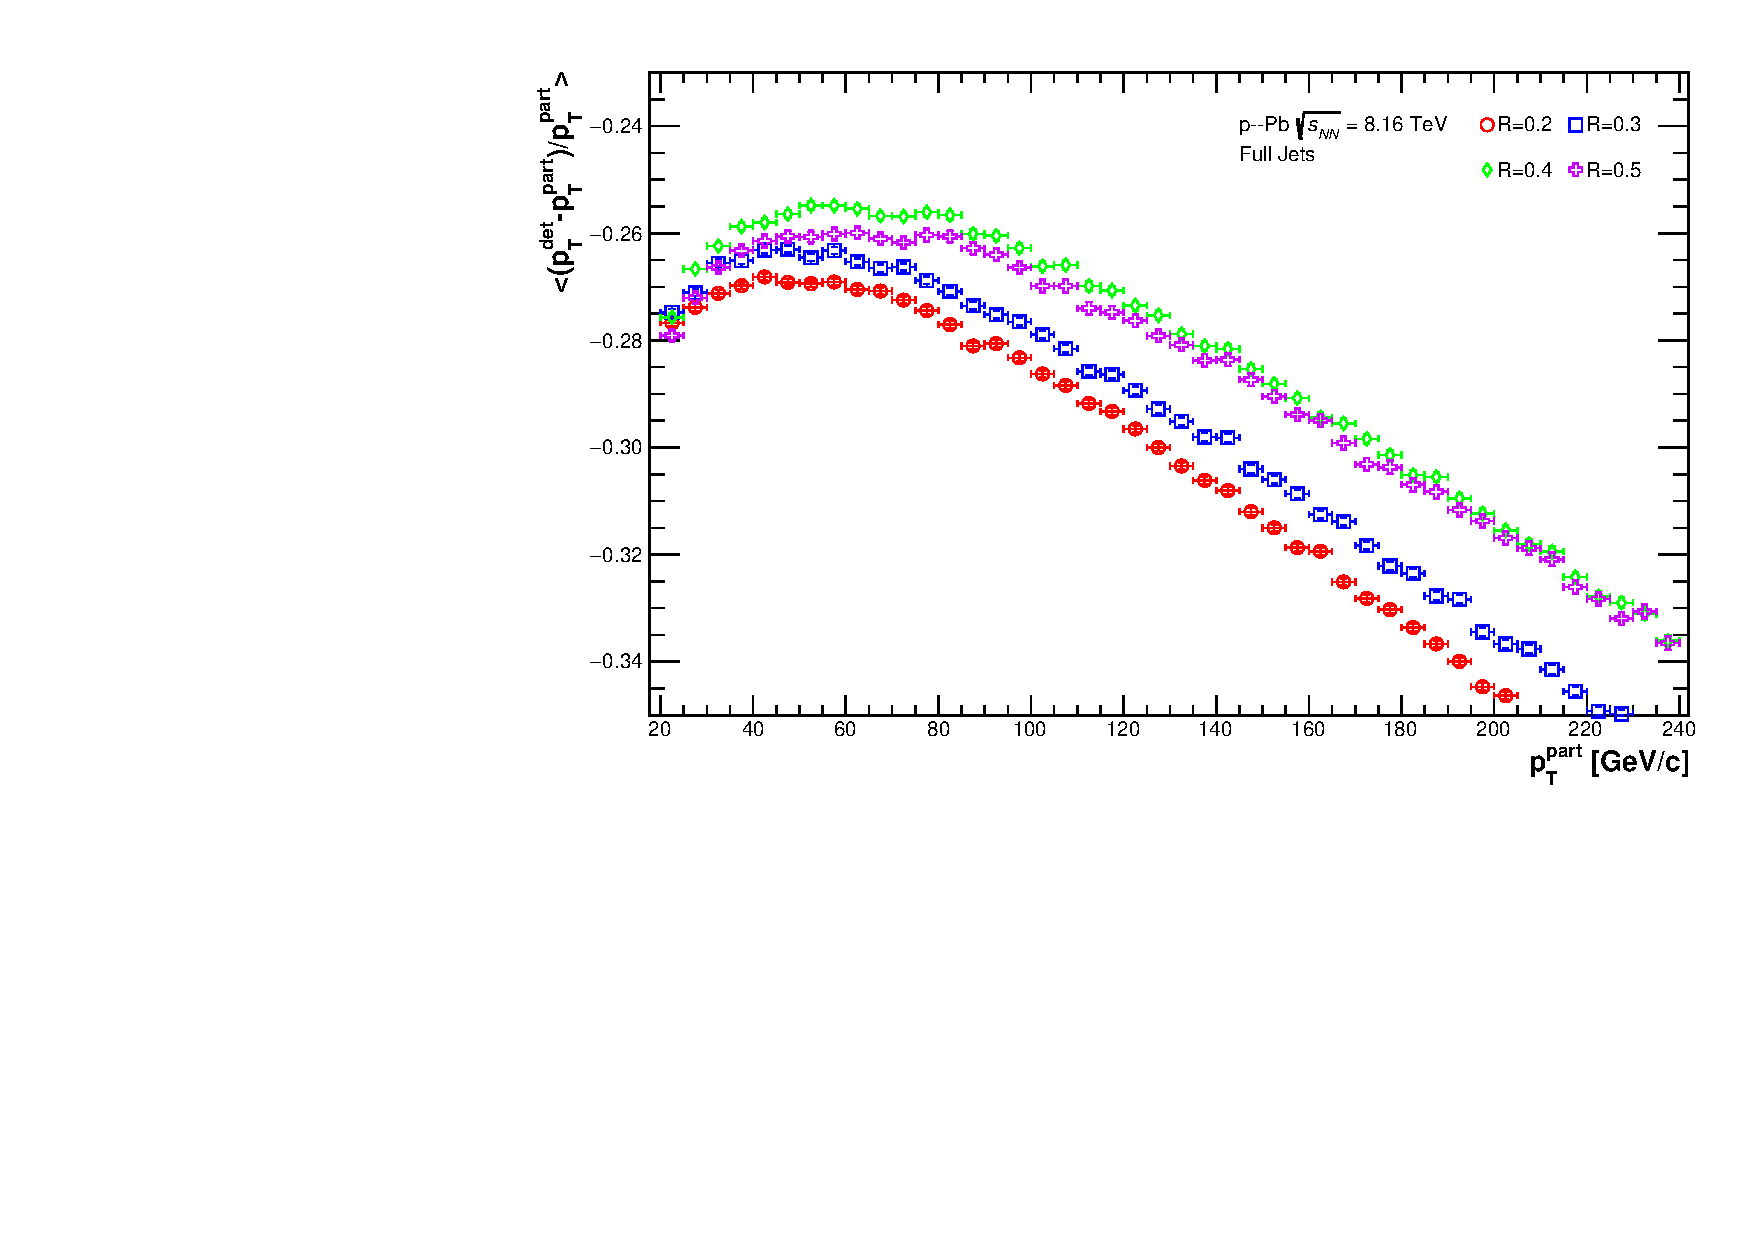
\includegraphics[width=7.5cm]{figures/EnergyScale/EnergyScaleMean.pdf}
        \vfill\null 
        \columnbreak
            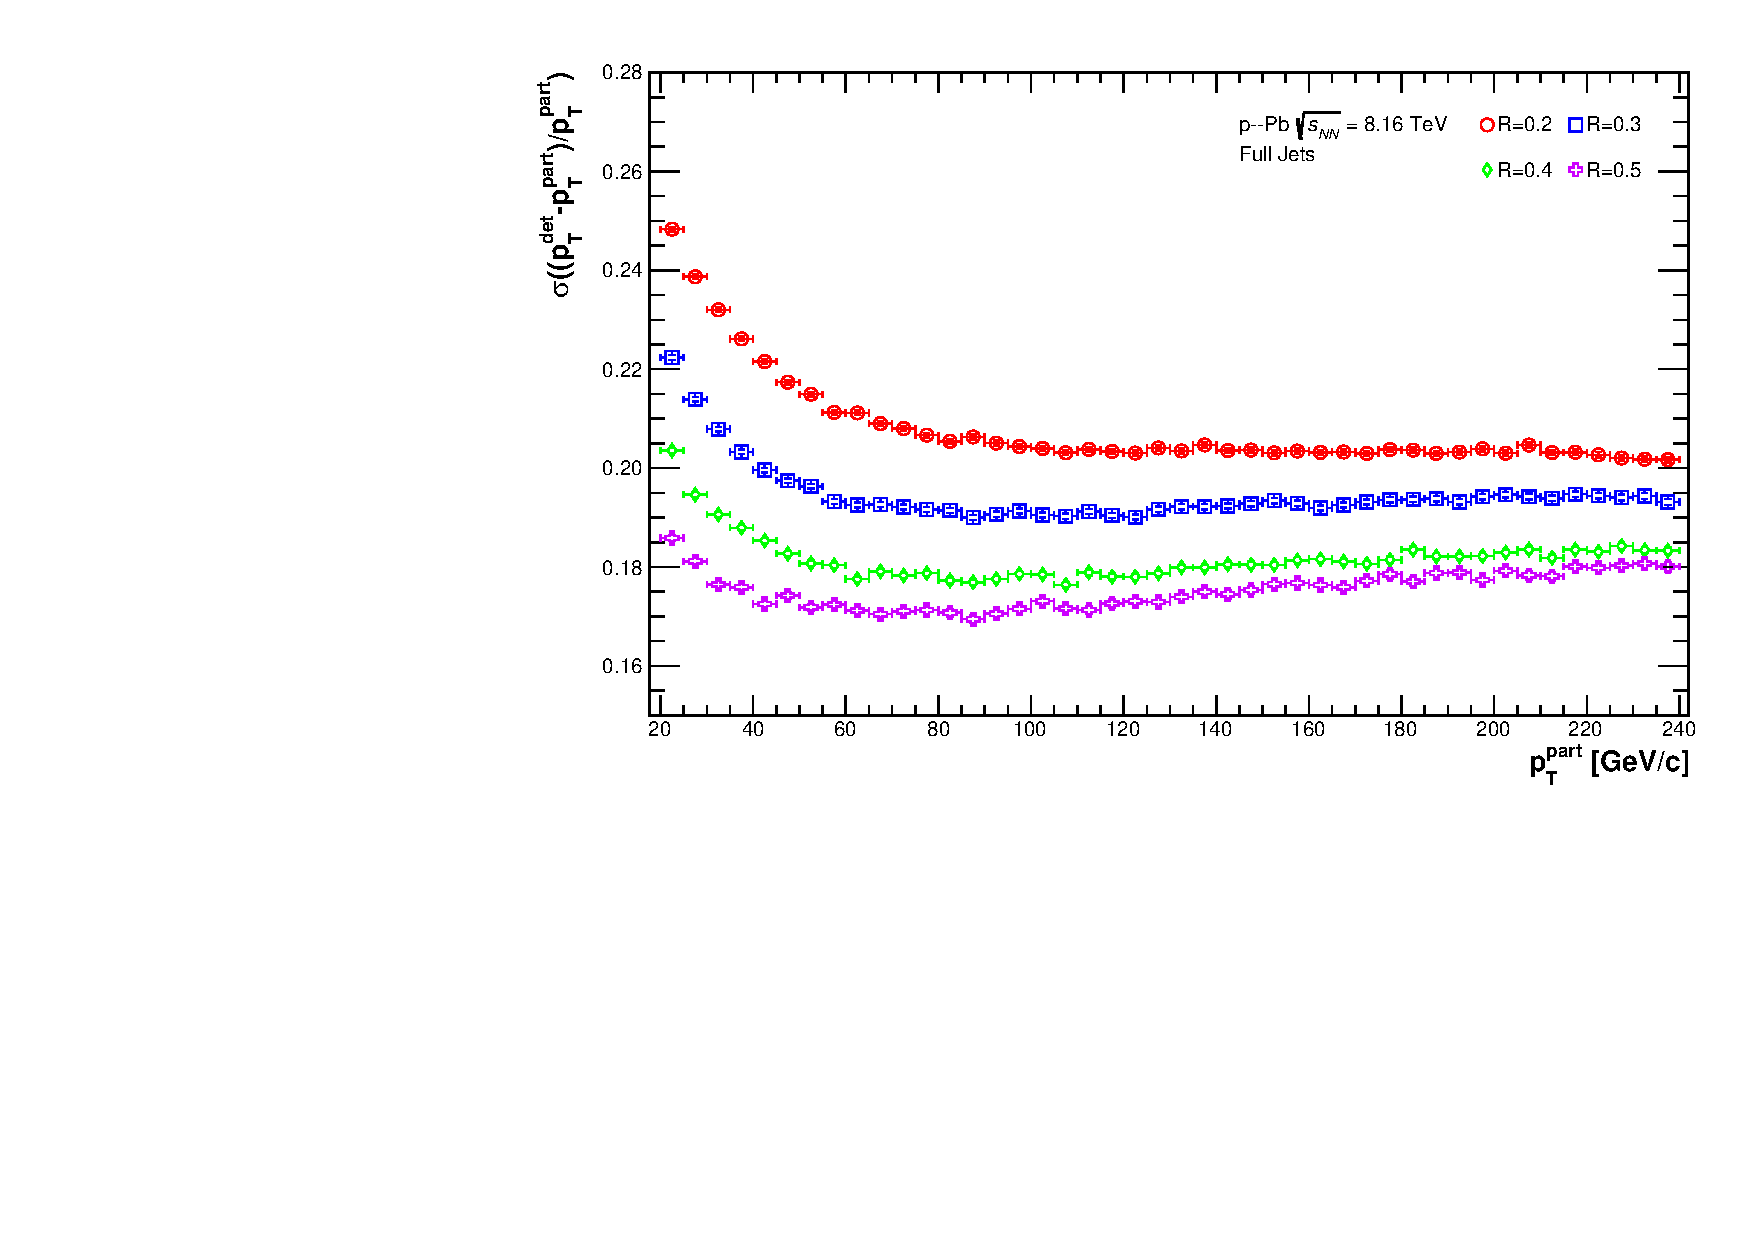
\includegraphics[width=7.5cm]{figures/EnergyScale/EnergyScaleWidth.pdf}
        \vfill\null
    \end{multicols}
    \caption{Jet energy scale (left) and jet energy resolution (right) showing the instrumental response for jets in \pp collisions.}
    \label{fig:EnergyScale}
\end{figure}

\begin{figure}[h!]
    \centering
    \begin{multicols}{2}
            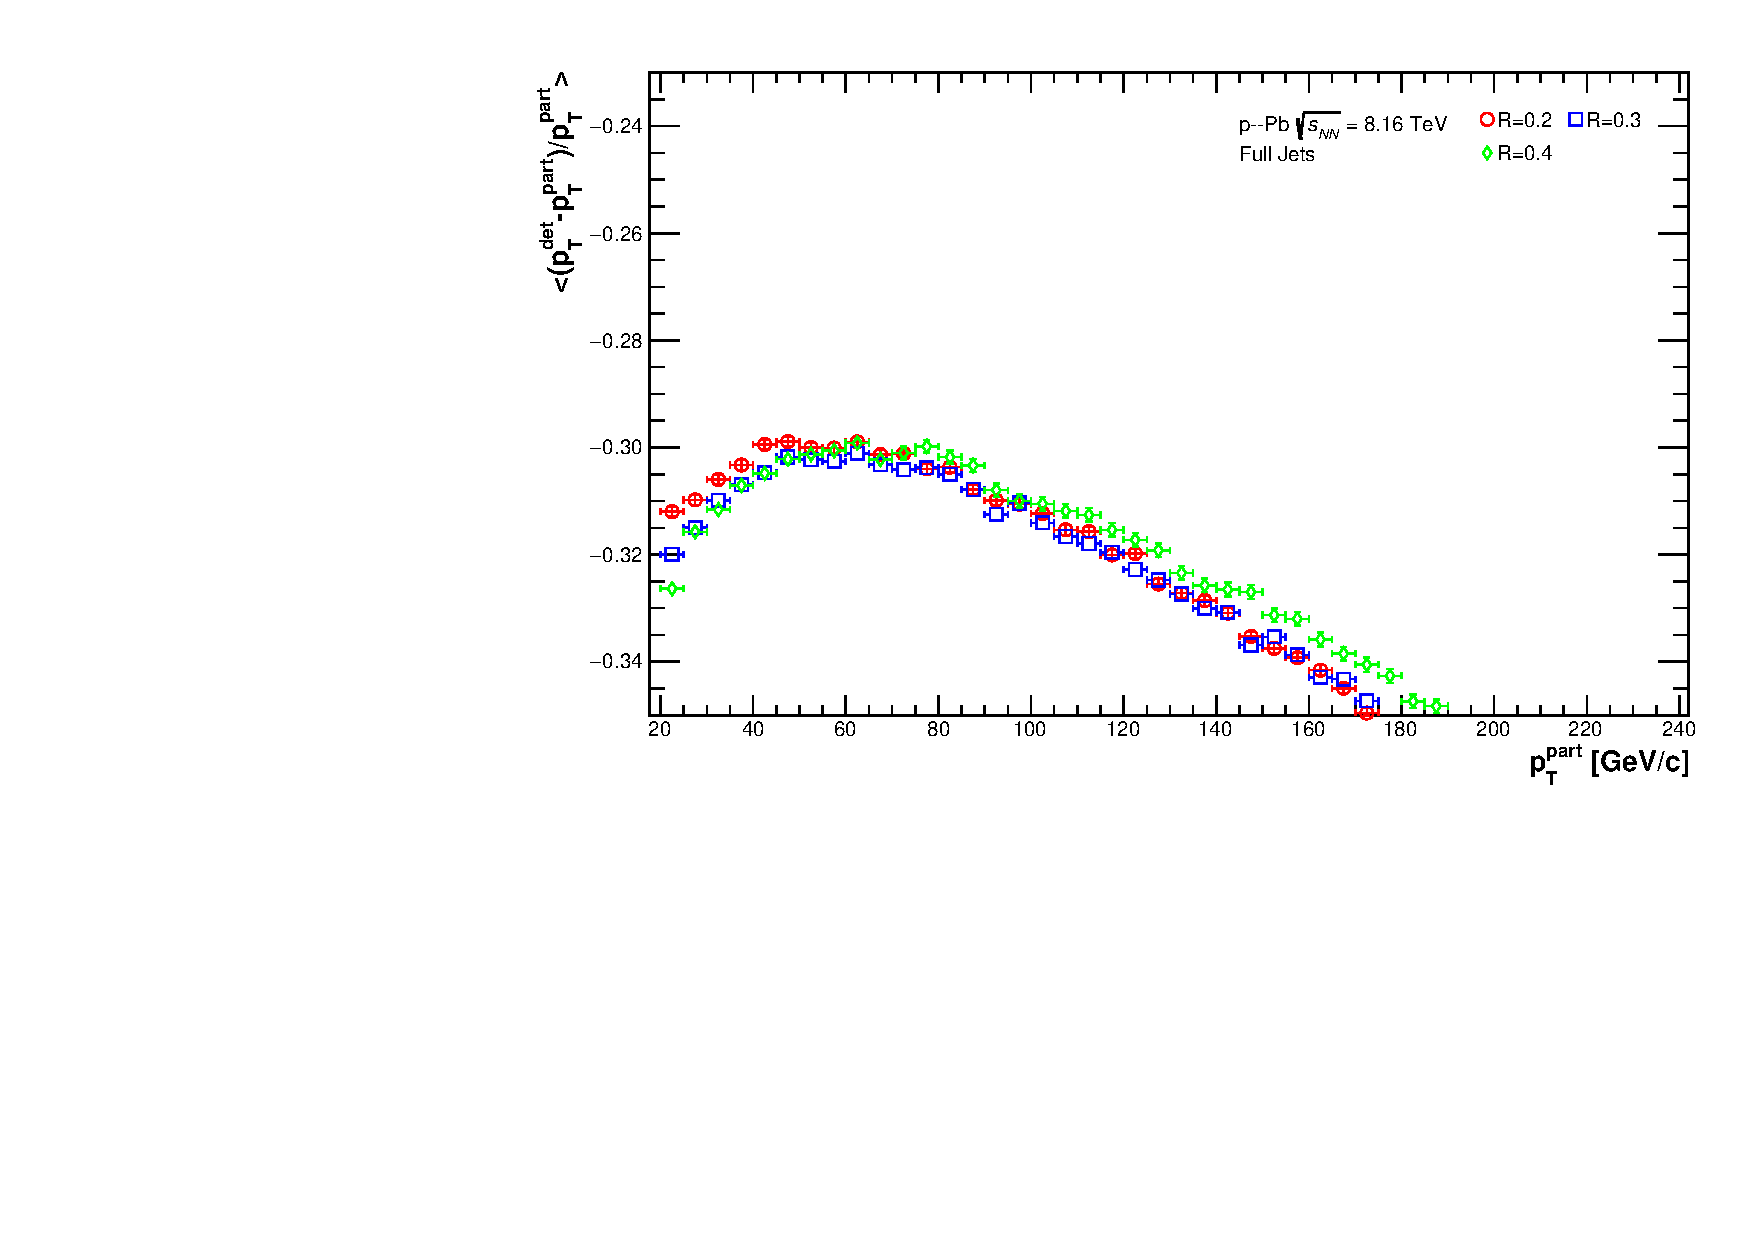
\includegraphics[width=7.5cm]{figures/pPbFigures/EnergyScale/EnergyScaleMean.pdf}
        \vfill\null 
        \columnbreak
            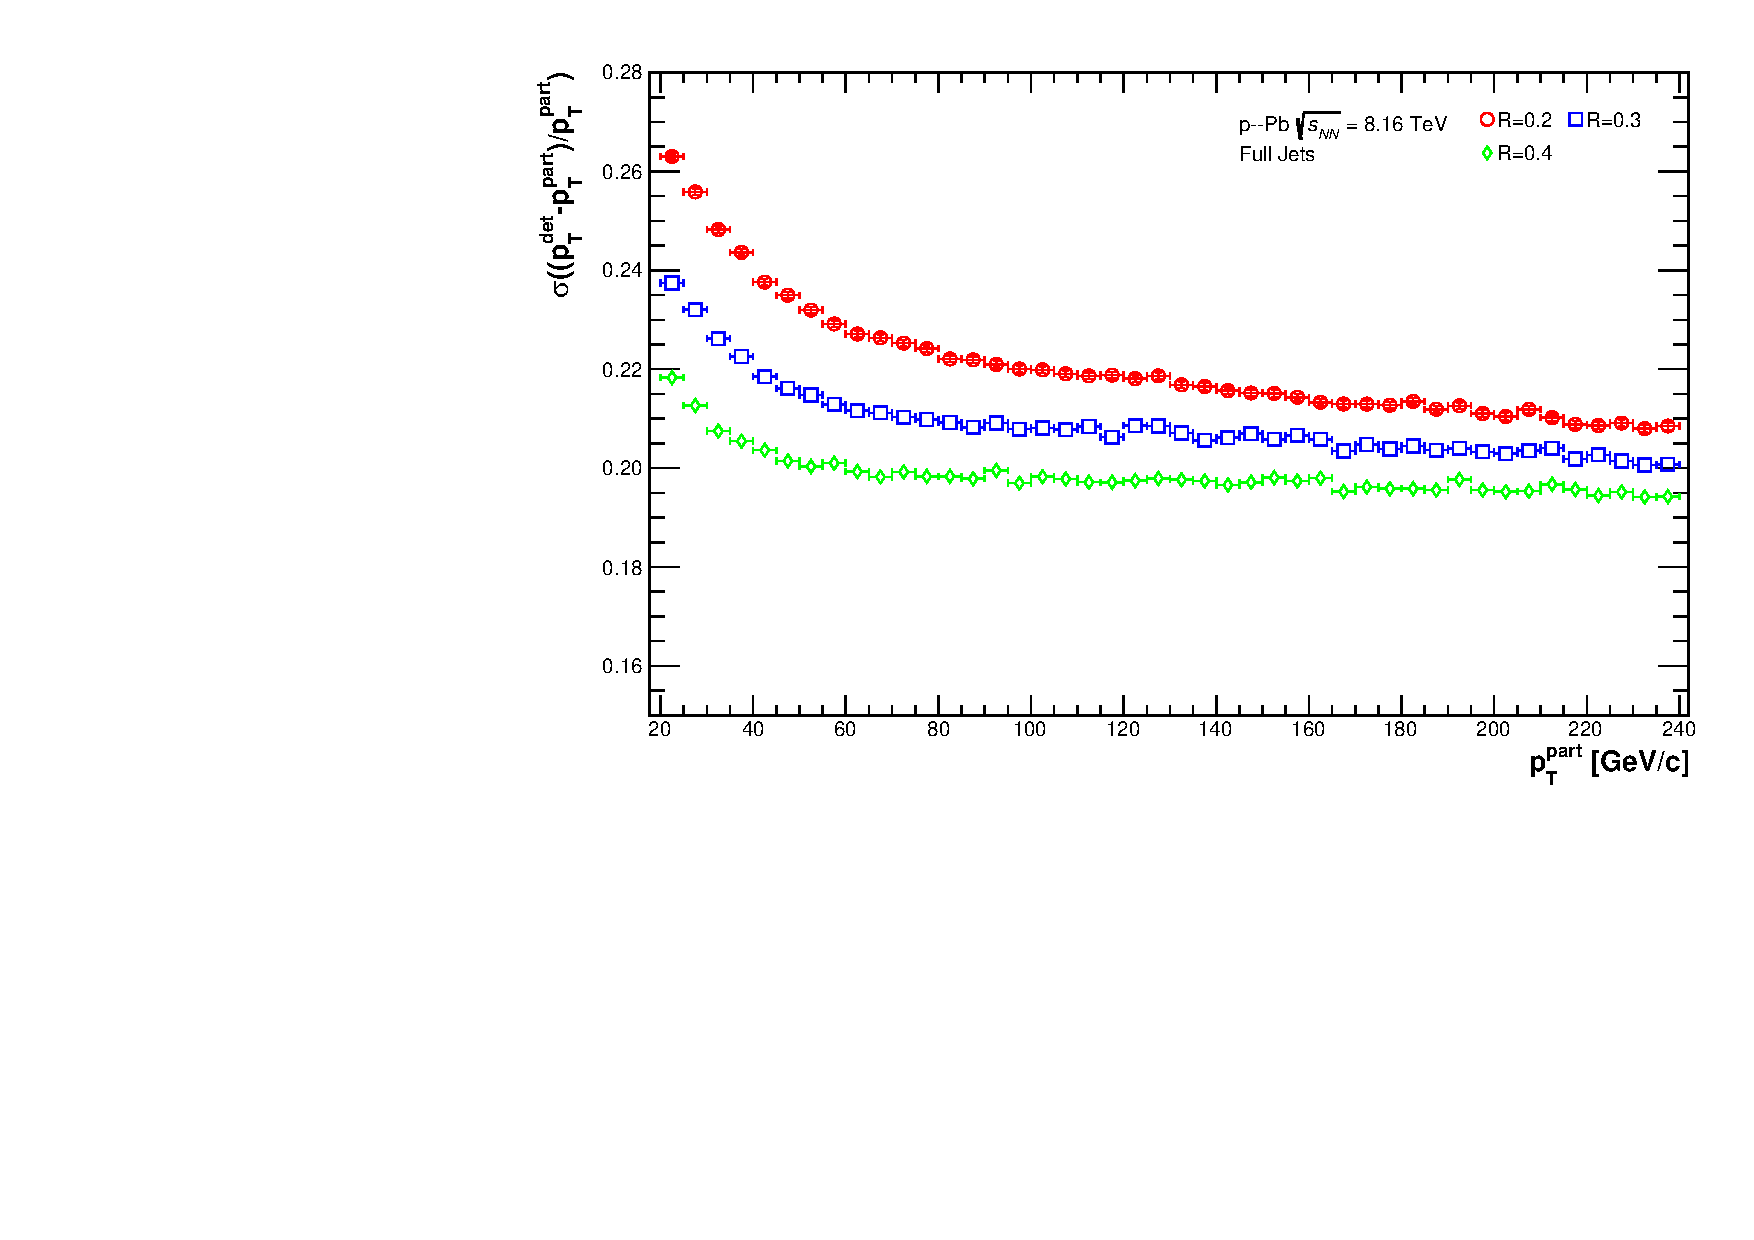
\includegraphics[width=7.5cm]{figures/pPbFigures/EnergyScale/EnergyScaleWidth.pdf}
        \vfill\null
    \end{multicols}
    \caption{Jet energy scale (left) and jet energy resolution (right) showing the instrumental response for jets in \pPb collisions.}
    \label{fig:EnergyScalepPb}
\end{figure}

In order to quantify the detector effects on the observables, the PYTHIA production LHC16c2 was used for \pp, and the PYTHIA productions LHC23d7a and LHC23d7b were used for \pPb. Generated events were fully propagated using GEANT3 to form a detector response in \pT$^{jet}$, which is used to unfold the measured jet distributions (see section \ref{sec:unfolding}). In order to account for background fluctuations in \pPb events, the response matrix for \pPb was smeared by the delta-\pT distribution from random cones. This method is further described in section 4.1.1 of \cite{anaNoteHHassan}. The instrumental response for \pp collisions is characterized in Fig. \ref{fig:EnergyScale}, while that for \pPb collisions can be found in Fig. \ref{fig:EnergyScalepPb}. The left plot shows the jet energy scale shift, quantified as the mean of the residuals distribution, as function of the true jet \pT. We see a mild R dependence and a relative negative shift of around 27\% at \pT$^{jet}$ = 100 GeV/c due to finite tracking efficiency. The right plot shows the jet energy resolution, quantified as the RMS of the residuals distribution. We observe that the jet energy resolution is relatively flat for full jets at higher \pT due to the neutral constituents.

For \pp, a comparison to the energy scale results from 13 TeV is also included, and can be seen in figure \ref{fig:EnergyScaleComp}. The larger the jet radius, the larger the difference gets compared to 13 TeV. This is likely due to detector performance effects. The performance for run 2 is significantly different, in part from a better resolution due to the inclusion of TRD tracking in ~50\% of events. Additionally, there was a smaller fraction of bad channels in the EMCal for run 2.

\begin{figure}[h!]
    \centering
    \begin{multicols}{2}
            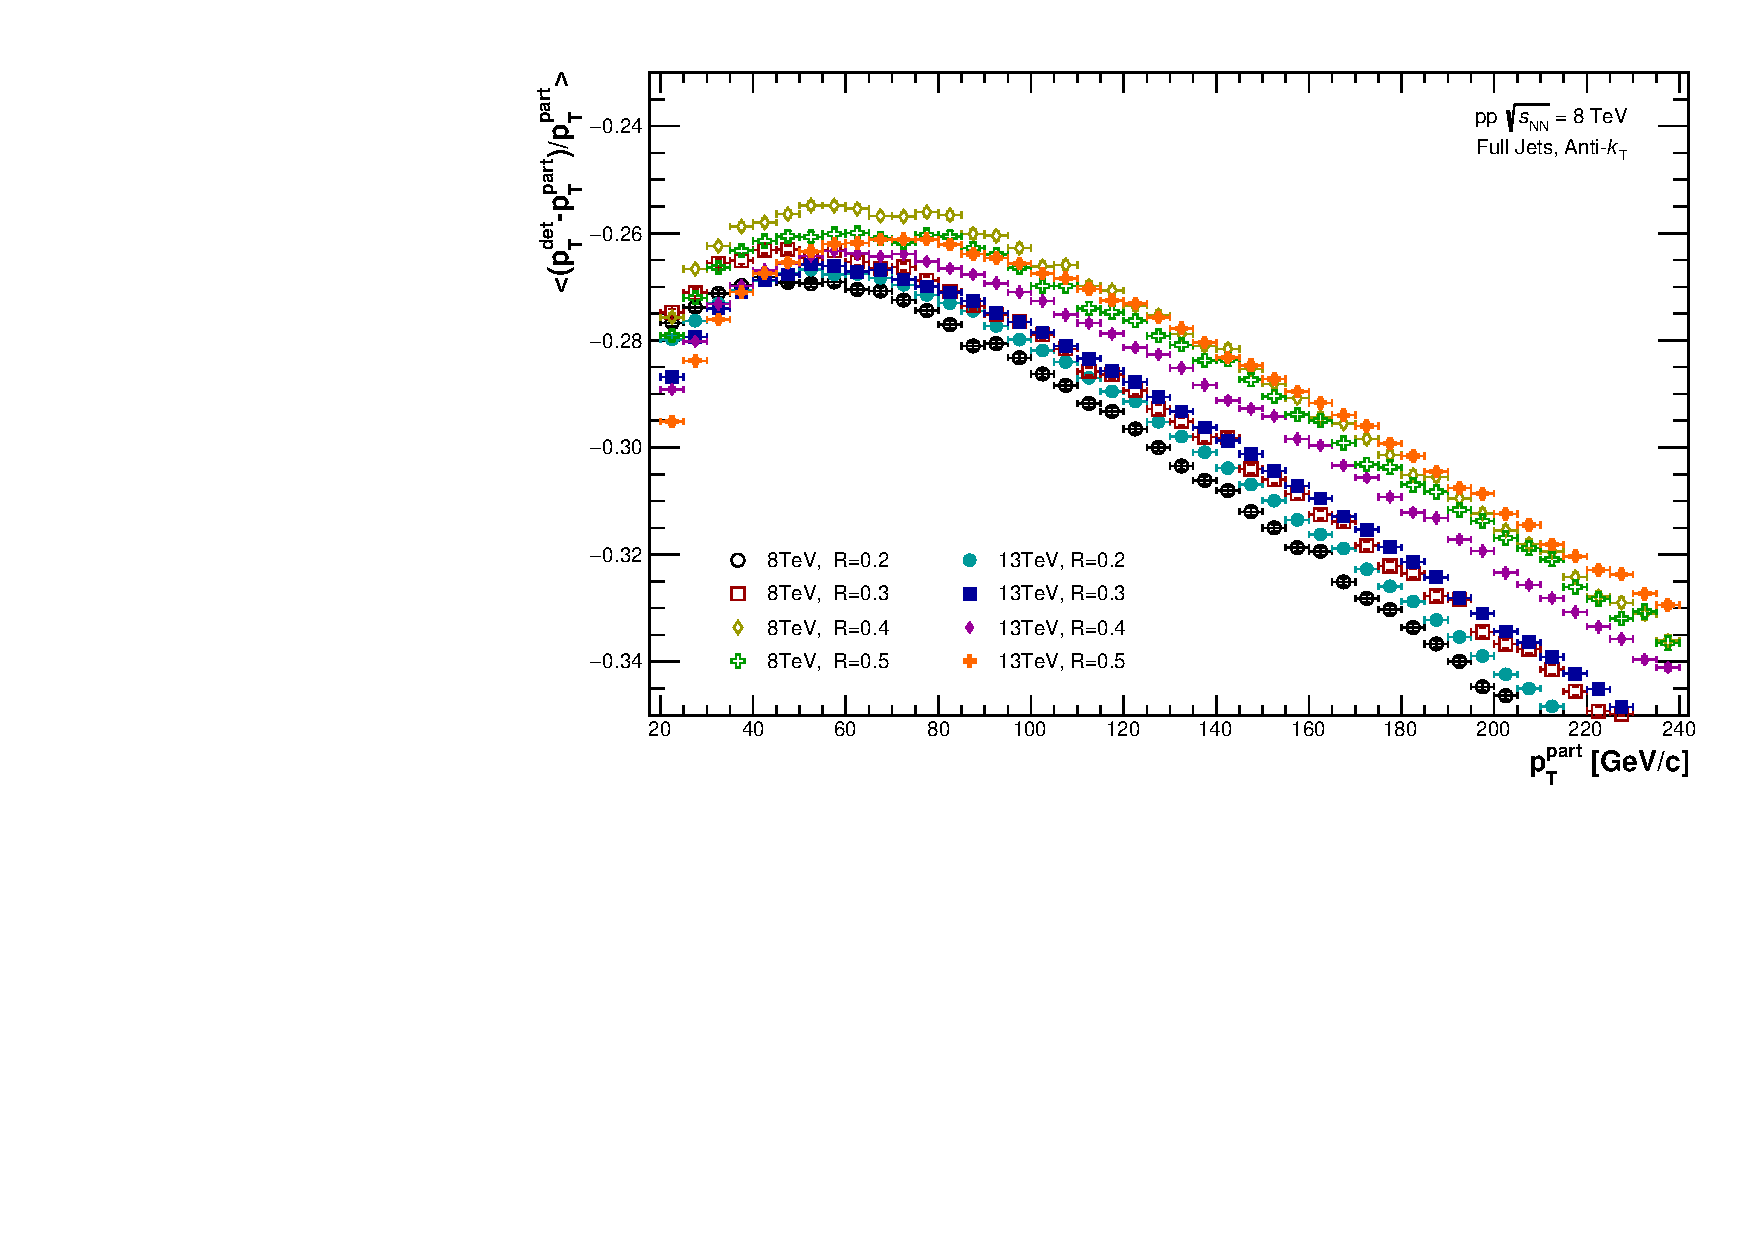
\includegraphics[width=7.5cm]{figures/EnergyScale/EnergyScaleMean_Comparison.pdf}
        \vfill\null 
        \columnbreak
            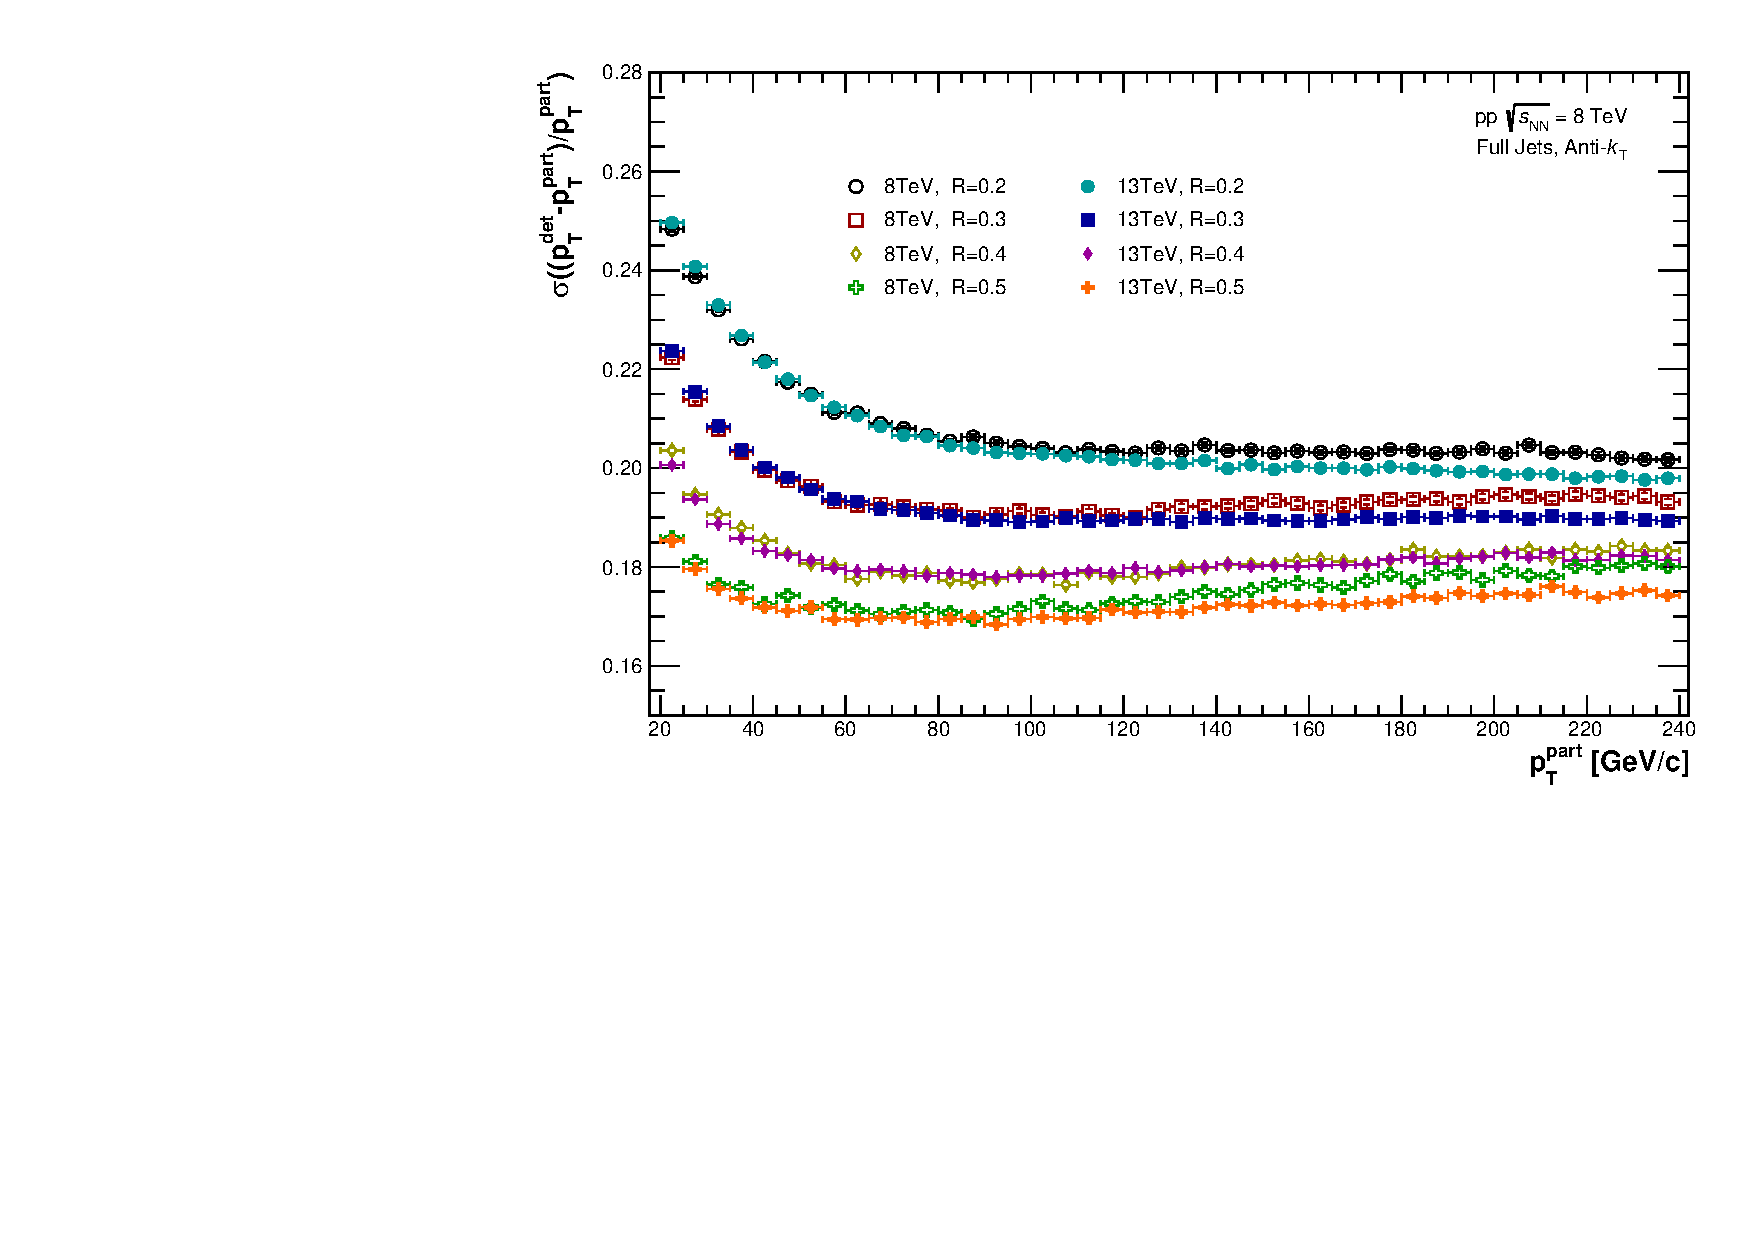
\includegraphics[width=7.5cm]{figures/EnergyScale/EnergyScaleWidth_Comparison.pdf}
        \vfill\null
    \end{multicols}
    \caption{Jet energy scale (left) and jet energy resolution (right) from the results of this analysis (\pp 8 TeV) compared to those of the \pp 13 TeV analysis.}
    \label{fig:EnergyScaleComp}
\end{figure}

A different R-ordering can also be seen when comparing the jet energy scale from 8 TeV and 13 TeV. For 13 TeV (and \pp 5 TeV), the energy scale increases with increasing radii from R = 0.2 - 0.6, whereas in 8 TeV, the energy scale increases from R = 0.2 - 0.4, then decreases again for R = 0.5 and R = 0.6. This has been studied, and a likely conclusion has been reached, but it is important to point out that although the jet energy scale ordering is different, it can be seen in figure \ref{fig:eScaleShapeWidth} that the shape of the distributions is comparable, but the width is slightly greater for 8 TeV.

\begin{figure}[h!]
    \centering
    \subfigure{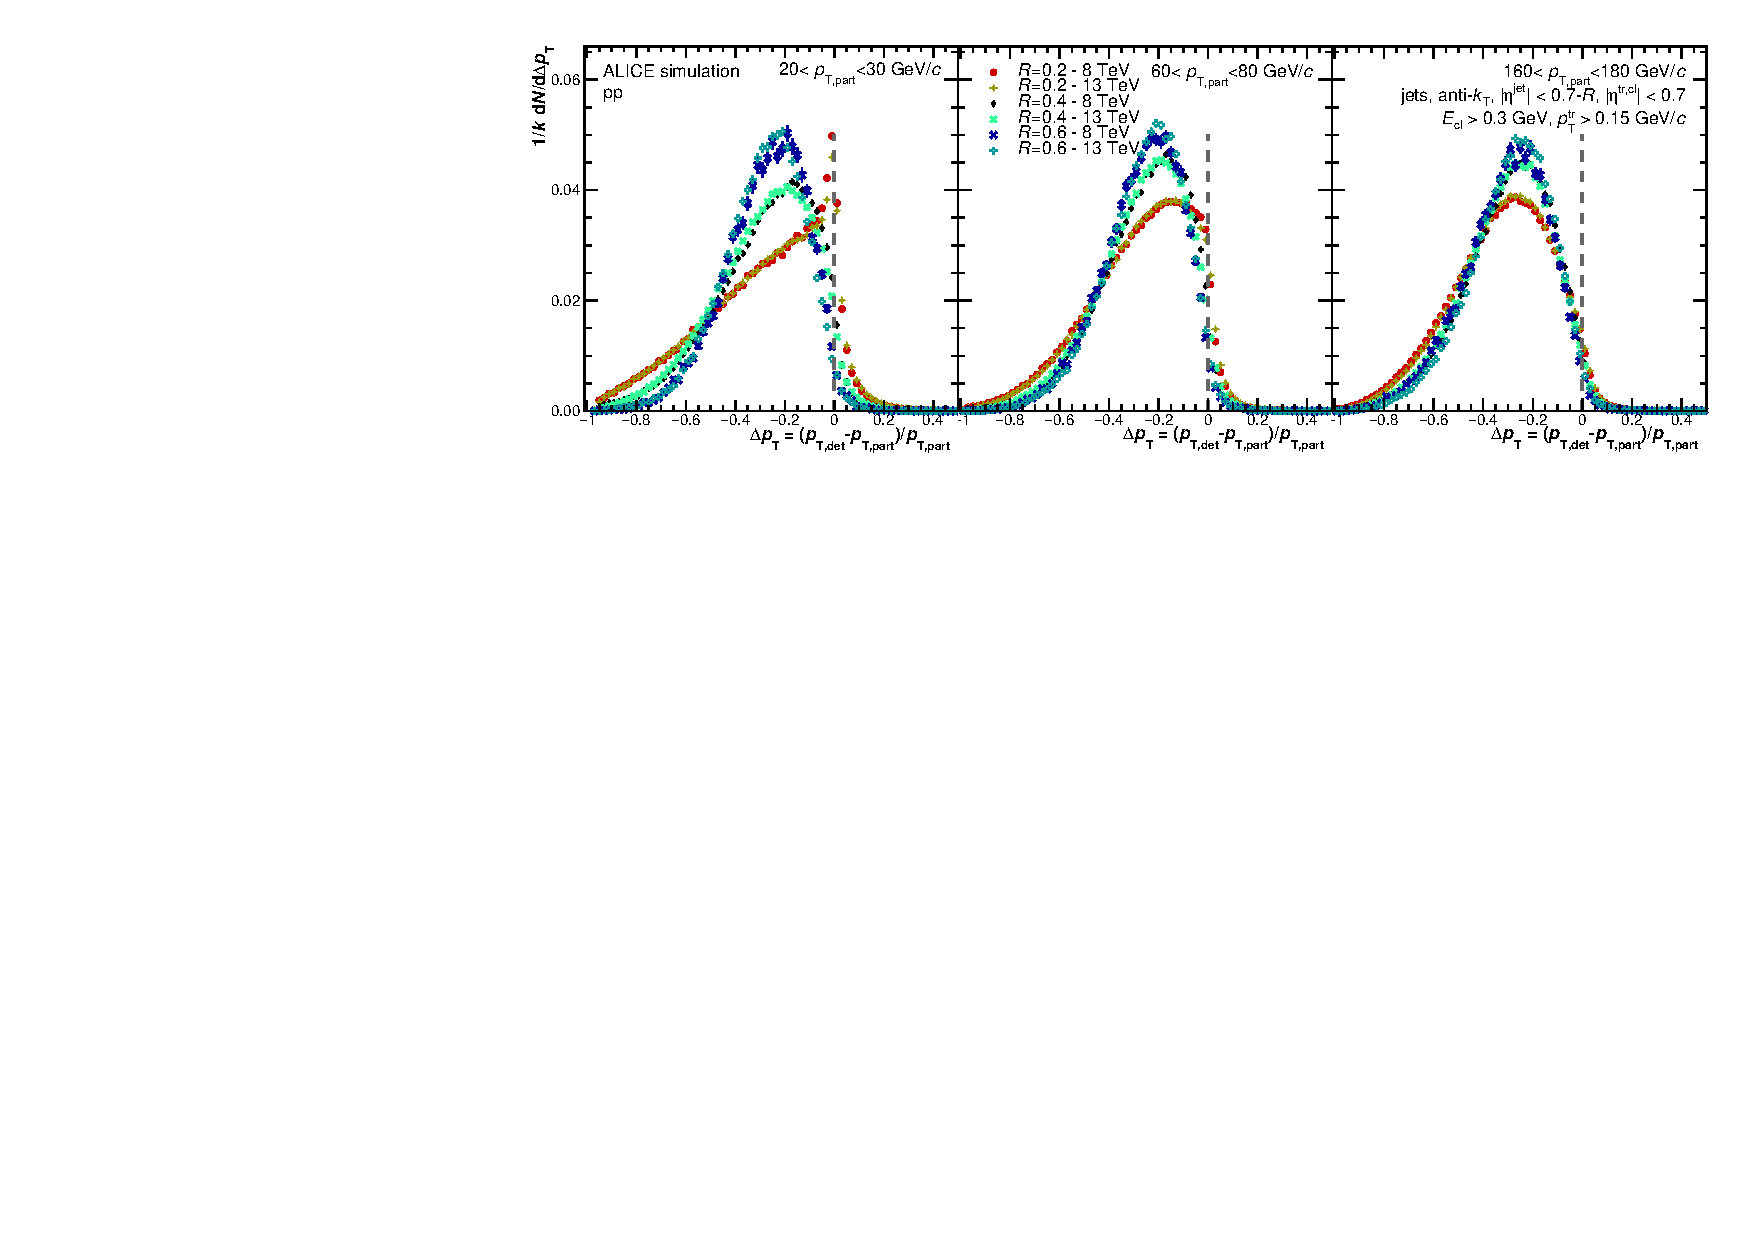
\includegraphics[width=0.85\textwidth]{figures/EnergyScale/ROrdering/JetEscaleProj_3_EnergyComp.pdf}}
    \subfigure{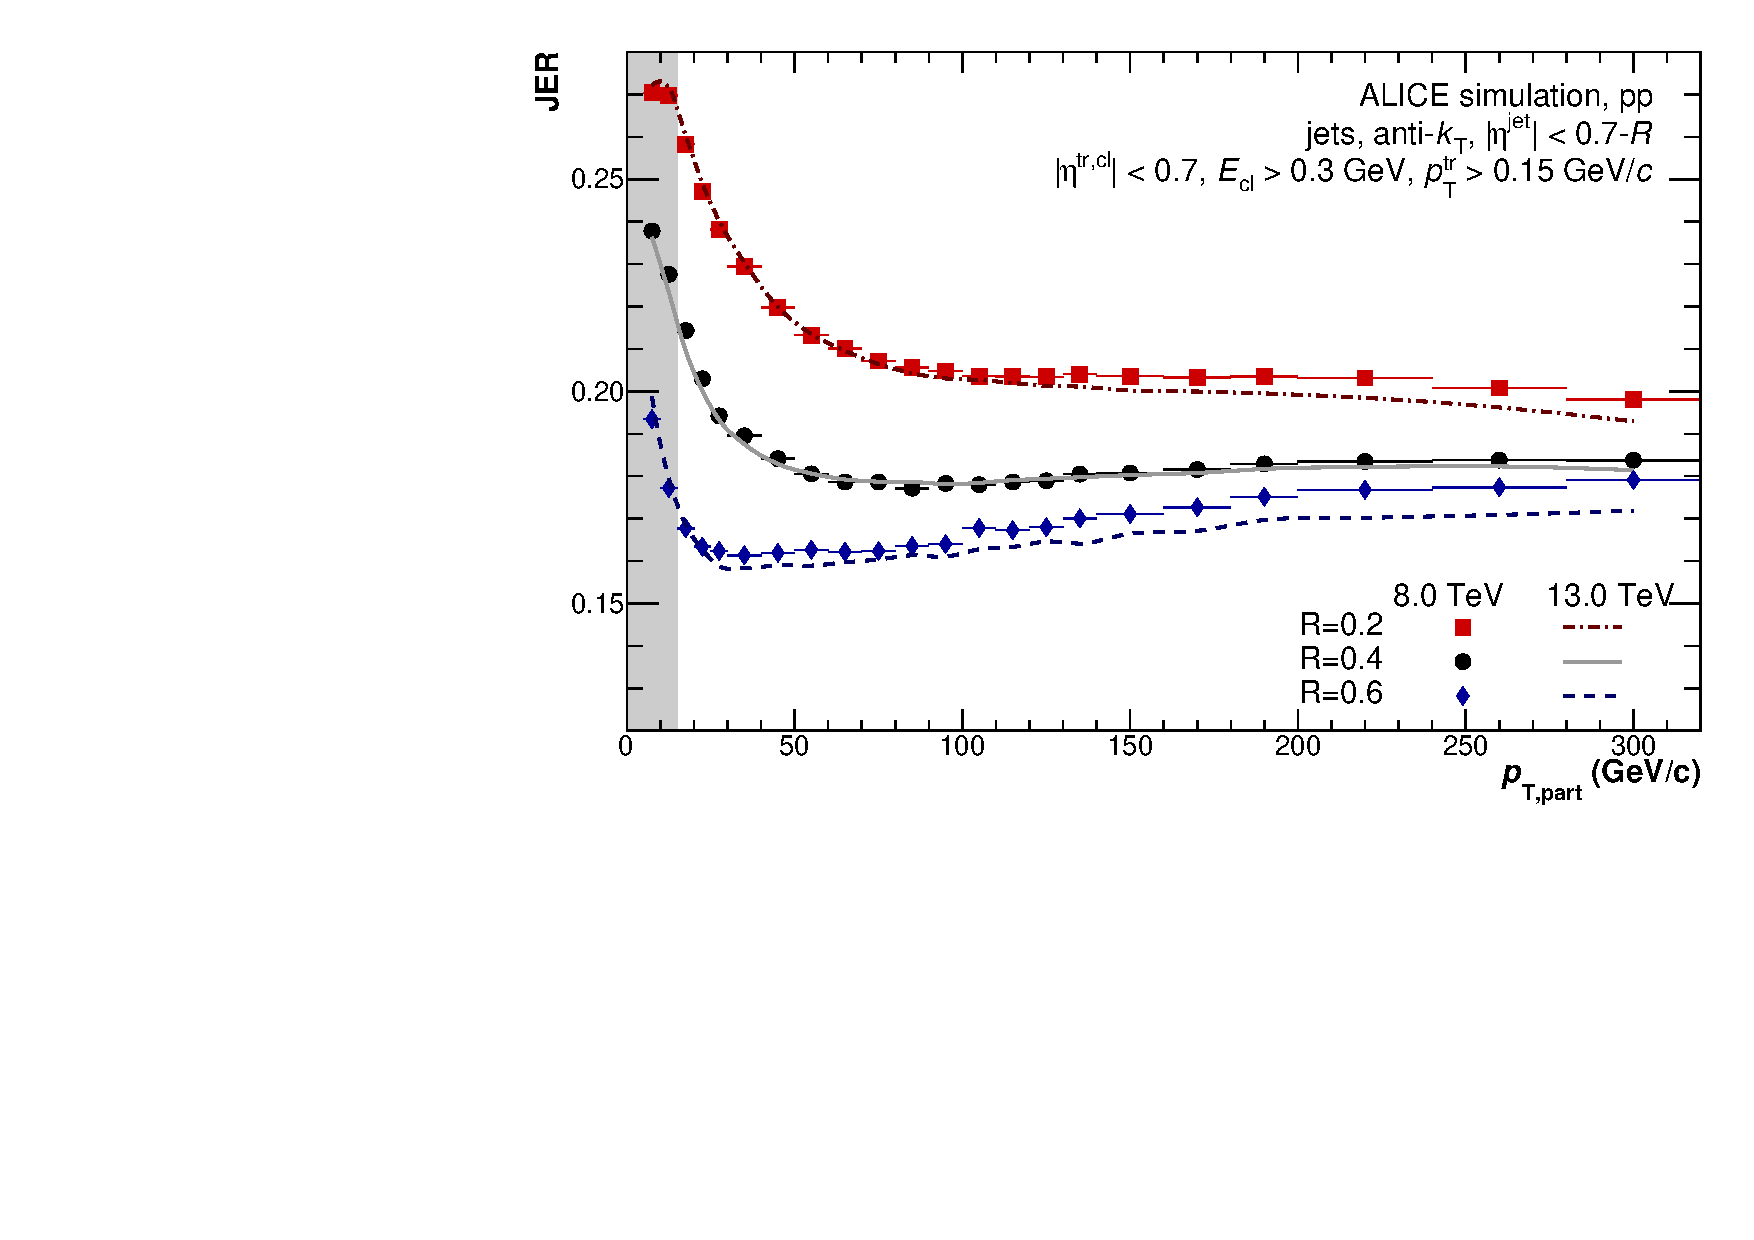
\includegraphics[width=0.75\textwidth]{figures/EnergyScale/ROrdering/JER_8_13_3_EnergyComp.pdf}}
    \caption{Jet energy scale projections showing the shape of the distributions (top), and the width of the residuals (bottom) for 8 and 13 TeV in \pp collisions.}
    \label{fig:eScaleShapeWidth}
\end{figure}

To explore the discrepancy, the jet energy scale is broken down into its charged and neutral components (figure \ref{fig:eScaleChNe}). The R-ordering difference is seen for both components, but is greater for the neutral component. For the charged component, in 2012, there were "holes" in the SPD tracking, and the ITS-TPC track matching was different as a function of phi. This was not present for the majority of the runs (evident by the smaller impact compared to the neutral component), but was enough to see an effect. For the neutral component, in 2012, the TRD was only partially installed. Some of the EMCal supermodules had TRD material in front of them, while others did not. The larger the jet radius, the more likely it was to cross boundaries in the EMCal between where there was and was not TRD material, or overlap with tracking holes in the ITS. Example plots showing tracking and EMCal occupancy as a function of $\eta$ and $\phi$ can be seen in figure \ref{fig:eScaleTracksClusters}.

\begin{figure}[h!]
    \centering
    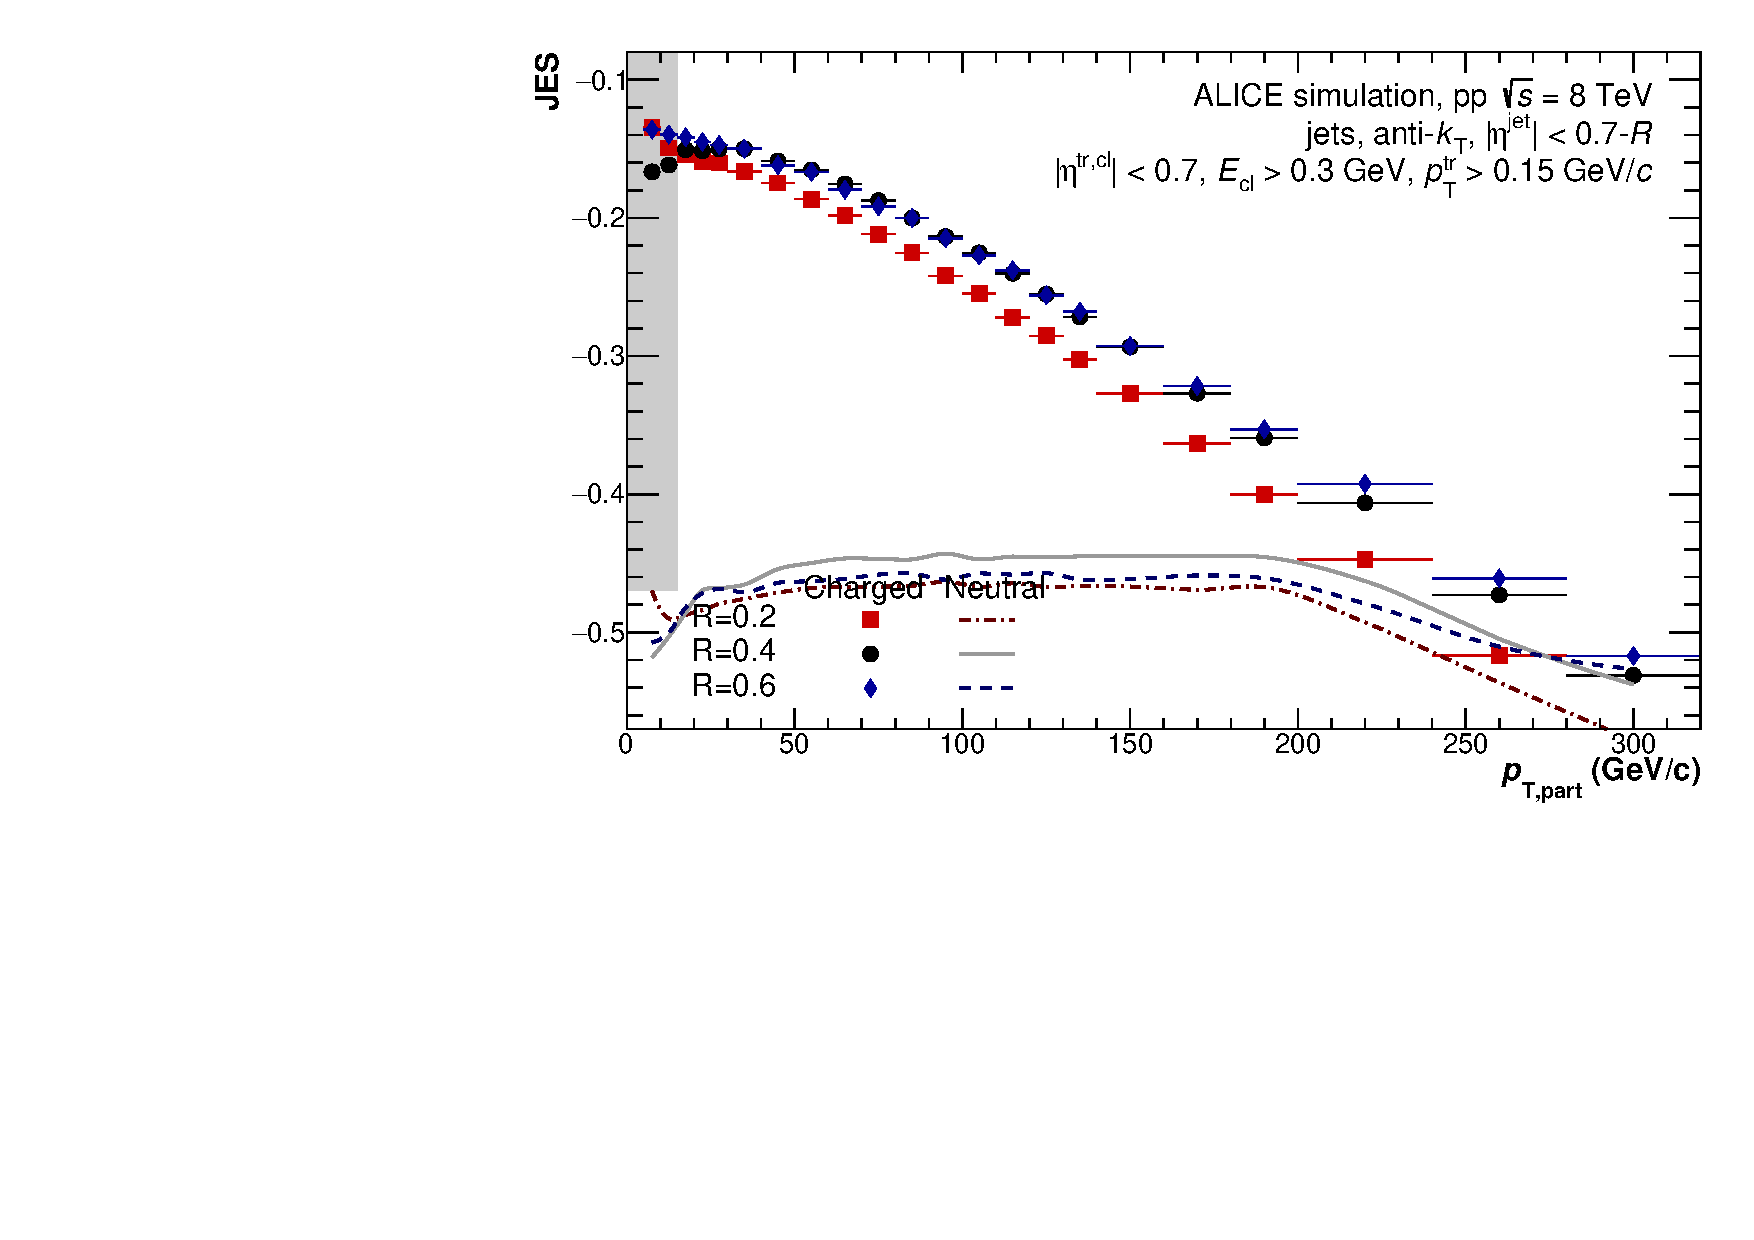
\includegraphics[width=0.75\textwidth]{figures/EnergyScale/ROrdering/JES_8_3_ChNe.pdf}
    \caption{Jet energy scale broken up into its charged and neutral components.}
    \label{fig:eScaleChNe}
\end{figure}

\begin{figure}[h!]
    \centering
    \subfigure{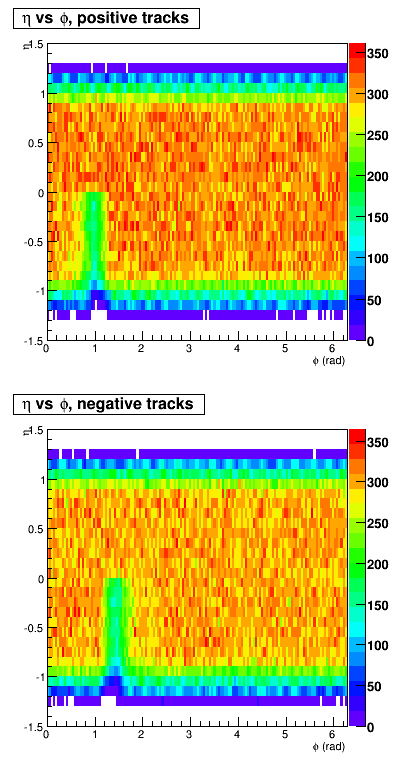
\includegraphics[width=0.25\textwidth]{figures/EnergyScale/ROrdering/spd_holes.png}}
    \subfigure{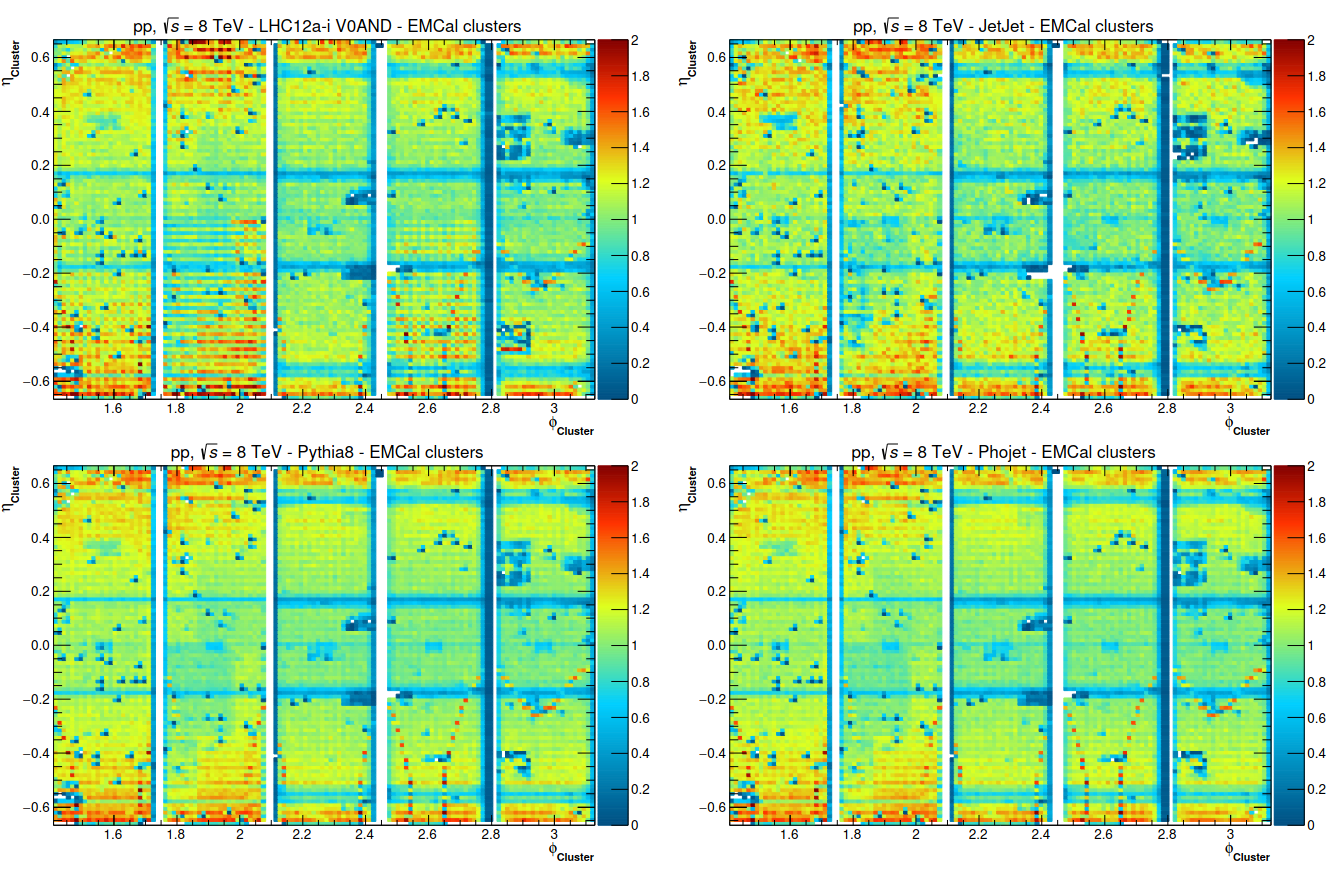
\includegraphics[width=0.73\textwidth]{figures/EnergyScale/ROrdering/emcal_occupancy.png}}
    \caption{TPC-ITS tracking (left) and EMCal occupancy (right) as a function of eta and phi.}
    \label{fig:eScaleTracksClusters}
\end{figure}
